\chapter{回归}
\label{chap:regression}

预测房屋价格时，可以估计平均成交价，也可以给出预算所需的上分位数或价格分布。\term{回归}（regression）根据输入估计数值响应的这些条件特征。设训练集为$D_n=\{(\bm{x}_i,y_i)\}_{i=1}^{n}$，其中$\bm{x}_i\in\mathbb{R}^{d}$为输入，$y_i\in\mathbb{R}$为响应，预测函数记为$f$；响应也可以是次数等离散数值。

回归的计算起点可追溯到19世纪初的最小二乘法，“回归”这一名称则来自Galton在1886年对亲子身高的研究。1970年代的广义线性模型扩展了响应类型，1980年代的回归树表达条件分区，1990年代的支持向量回归及随后发展的树集成进一步容纳非线性与交互\scite{galton1886,nelder1972glm,breiman1984cart}

如今，需要检查变量作用或建立简洁基线时，线性模型仍是常见起点；面对复杂表格数据，随机森林与梯度提升树是常用候选。现代基准也表明，梯度提升树仍有竞争力，但表现取决于数据、调参与计算预算，不能据此认定一种模型总占优势\scite{erickson2026tabarena}

本章依次介绍基于线性关系、邻域、树与规则、概率和集成的回归：分别用全局加权、局部样本、条件分区、分布与后验、成员组合来预测响应。共享机制见第\ref{chap:classic-models-overview}章，这里展开各自的目标、学习过程与适用条件。

\section{基于线性关系的回归}
\label{sec:regression-linear}

第\ref{sec:classic-overview-linear}节的加权和在这里用于预测数值响应。本节从最小二乘开始，再通过正则化控制系数、通过损失选择均值或分位数目标、通过核扩展函数表示。广义线性模型与可加模型进一步改变响应分布或特征作用；高斯误差只属于其中的特定设定。

\subsection{普通最小二乘（OLS）}
\label{sec:regression-ols}

从样本中选择一组系数，需要先规定怎样衡量预测误差。\term{普通最小二乘}（ordinary least squares, OLS）选择使残差平方和最小的系数。它既可以作为一个无需指定响应分布的优化准则，也可以在高斯噪声模型下解释为最大似然估计；以下先建立前一种形式，再说明统计结论需要哪些额外条件\scite{bishop2006}

这种误差准则早于“回归”的名称。Legendre在1805年公开发表最小二乘法时，面对的是观测方程多于未知量、各方程通常无法同时精确成立的问题；误差平方和提供了在不一致观测之间取舍的准则。Gauss在1809年的天体轨道著作中又从观测误差的概率分析出发讨论其依据\scite{stigler1981,gauss1809}

\subsubsection{模型结构}
\label{sec:regression-ols-structure}

令$\bm{\phi}(\bm{x})\in\mathbb{R}^{p}$表示固定特征向量，模型写成$f_{\bm{w}}(\bm{x})=\bm{\phi}(\bm{x})^{\top}\bm{w}$，其中$\bm{w}\in\mathbb{R}^{p}$。最简单的选择是$\bm{\phi}(\bm{x})=(1,\bm{x}^{\top})^{\top}$，此时$p=d+1$，第一个系数为截距。这里的“线性”指预测对待估计系数线性；特征变换$\bm{\phi}$可以非线性，其具体形式将在本小节后面展开。

把样本堆叠为设计矩阵$\bm{X}\in\mathbb{R}^{n\times p}$，第$i$行为$\bm{\phi}(\bm{x}_i)^{\top}$，并记$\bm{y}=(y_1,\ldots,y_n)^{\top}$，得到目标
\begin{equation}
  \widehat{\bm{w}}\in\argmin_{\bm{w}}J(\bm{w}),
  \qquad
  J(\bm{w})=\frac{1}{2n}\lVert\bm{y}-\bm{X}\bm{w}\rVert_2^2.
  \label{eq:regression-ols-objective}
\end{equation}
因子$1/(2n)$不改变OLS的最优解，但会影响梯度、步长和正则系数的数值约定。本章使用平均平方损失时均沿用这一形式。

图\ref{fig:regression-ols-residuals}把这个目标放回输入与响应平面：每条虚线都是固定$x_i$之后，观测$y_i$与直线预测之间的纵向差。OLS选择的是让这些差的平方和最小的直线，因此拟合线通常不穿过每个样本；这里测量的也不是点到直线的垂直几何距离。

\begin{figure}[htbp]
  \centering
  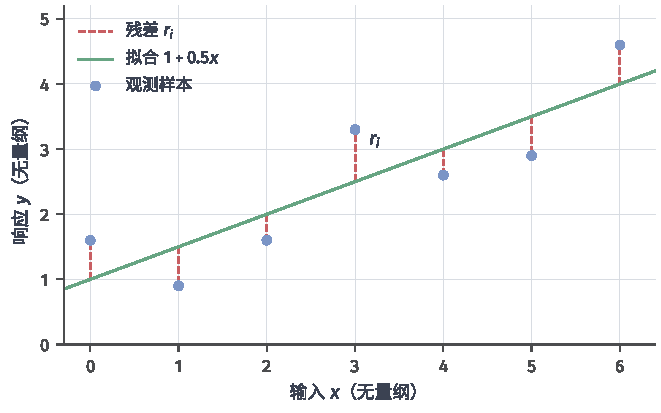
\includegraphics[width=\linewidth]{figures/03-models/01-classic-models/matplotlib/regression-ols-residuals/figure.pdf}
  \caption{一维OLS与响应残差。七个构造样本的最小二乘直线为$\widehat f(x)=1+0.5x$；蓝色实心点表示观测，绿色实线表示预测，红色竖虚线表示$r_i=y_i-\widehat f(x_i)$。横、纵轴均为无量纲教学变量。}
  \label{fig:regression-ols-residuals}
\end{figure}

平方损失的总体目标由
\BookTheoremRef{thm:probability-conditional-mean-l2-projection}{第一卷“数学准备”的条件均值最小平方误差定理}
确定：响应二阶矩有限时，条件均值在平方可积预测函数中达到最小风险，且只在输入分布的几乎处处意义下唯一。
限制为$f_{\bm w}$以后，若条件均值不属于所选模型类，OLS估计的只是该类中的平方逼近；
高斯性、同方差性与误差对称性都不是平方损失以条件均值为目标的必要条件。

\subsubsection{参数学习}
\label{sec:regression-ols-learning}

目标的梯度为$\bm{X}^{\top}(\bm{X}\bm{w}-\bm{y})/n$，Hessian为$\bm{X}^{\top}\bm{X}/n$，后者半正定。因此使梯度为零既是必要条件，也是充分条件，得到\term{正规方程}（normal equations）：残差与每一列特征都正交。
\begin{equation}
  \bm{X}^{\top}\bm{X}\widehat{\bm{w}}=\bm{X}^{\top}\bm{y}.
  \label{eq:regression-normal-equations}
\end{equation}

\BookTheoremRef{thm:matrix-analysis-pseudoinverse-minimum-norm}{第一卷“数学准备”的“最小二乘与最小范数”定理}
给出全部参数解$\bm X^\dagger\bm y+\operatorname{null}(\bm X)$。
因此训练拟合值总是唯一，参数唯一则要求设计矩阵列满秩；否则可取最小范数解。
零空间中的参数差在训练点上不可见，却可能在新特征向量上产生不同预测。

闭式表达用于分析，计算时通常不显式求逆。列满秩且$n\geq p$时，薄QR分解$\bm{X}=\bm{Q}\bm{R}$把问题化为三角方程$\bm{R}\widehat{\bm{w}}=\bm{Q}^{\top}\bm{y}$，稠密计算代价约为$O(np^2)$。秩亏或需要检查小奇异值时可以用SVD。直接形成$\bm{X}^{\top}\bm{X}$会把满列秩矩阵的二范数条件数平方，因此近似共线时尤其应避免求逆实现。

当矩阵分解不便进行时，可迭代更新
\begin{equation}
  \bm{w}^{(t+1)}
  =\bm{w}^{(t)}+\frac{\eta}{n}
       \bm{X}^{\top}(\bm{y}-\bm{X}\bm{w}^{(t)}).
  \label{eq:regression-ols-gradient}
\end{equation}
一次完整更新需要$O(np)$次算术操作；使用大小为$b$的小批量时，一次梯度估计需$O(bp)$，但总更新次数和随机误差也须考虑。代码\ref{code:regression-ols}展示矩阵求解接口与预测；截距列需由调用者加入，返回的秩可用于检查参数是否可识别。

\begin{codeblock}[language=Python,label={code:regression-ols},unbreakable]{用最小二乘接口求解并预测}
import numpy as np

# X: (n, p), y: (n,), X_new: (n_new, p)
# 截距列与特征变换在训练、预测时保持一致。
w, residuals, rank, singular_values = np.linalg.lstsq(
    X, y, rcond=None
)
y_pred = X_new @ w
\end{codeblock}

\subsubsection{理论分析}
\label{sec:regression-ols-theory}

OLS的计算结论与统计结论依赖不同的随机性。固定设计下可以分别考察优化误差和参数估计误差；转到独立同分布的随机设计，讨论的则是估计量的渐近分布。下面得到的结论包括确定性收敛、条件均方误差和依概率或依分布的极限，但不能据此保证模型失配或任意测试分布下的风险。

\paragraph{收敛性分析}
式\eqref{eq:regression-ols-gradient}是
\BookTheoremRef{thm:gradient-descent-minimum-norm}{第一卷“数学准备”的最小二乘梯度迭代选解定理}
在平均损失归一化下的应用。令$\bm A=\bm X^\top\bm X/n$，当$\bm X\ne\bm0$且
$0<\eta<2/\lambda_{\max}(\bm A)$时，非零谱方向收敛；秩亏时零空间分量保持初值，
从零启动得到最小范数解。这个结论针对固定训练目标，不保证新样本风险；
归一化改变了允许的学习率尺度，不能直接照搬未平均目标的步长。

\paragraph{泛化分析}
求到经验最优解后，还需考察有限样本造成的估计误差及其对新输入预测的影响。偏差与方差分析需要指定响应如何产生。以下条件于固定设计，假设
\begin{equation}
  \bm{y}=\bm{X}\bm{w}_{\star}+\bm{\varepsilon},\qquad
  \mathbb{E}[\bm{\varepsilon}\mid\bm{X}]=\bm{0},\qquad
  \operatorname{Cov}(\bm{\varepsilon}\mid\bm{X})=\sigma^2\bm{I}_n,
  \quad 0<\sigma^2<\infty.
  \label{eq:regression-gauss-markov-model}
\end{equation}
这些条件要求均值模型正确、误差同方差且两两不相关；不相关不等于独立，也没有要求高斯分布。

\Needspace{9\baselineskip}
\begin{theorem}[Gauss--Markov定理]
  \label{thm:regression-gauss-markov}
  在式\eqref{eq:regression-gauss-markov-model}下，若$\bm{X}$列满秩，OLS无偏，协方差为$\sigma^2(\bm{X}^{\top}\bm{X})^{-1}$。对任何条件于$\bm{X}$固定、对所有$\bm{w}_{\star}$均无偏的线性估计$\widetilde{\bm{w}}=\bm{C}\bm{y}$，有
  \[
    \operatorname{Cov}(\widetilde{\bm{w}}\mid\bm{X})
    -\operatorname{Cov}(\widehat{\bm{w}}\mid\bm{X})\succeq\bm{0}.
  \]
\end{theorem}

\begin{proof}
条件于设计矩阵后，直接应用
\BookTheoremRef{thm:statistics-gauss-markov}{第一卷“数学准备”的Gauss--Markov定理}。
本节额外说明的是该协方差怎样影响新输入的回归预测。
\end{proof}

这里的“最优”限定在线性无偏估计的协方差比较中，不涉及所有预测算法。对固定新特征$\bm{\phi}_{\star}$，估计条件均值的均方误差为$\sigma^2\bm{\phi}_{\star}^{\top}(\bm{X}^{\top}\bm{X})^{-1}\bm{\phi}_{\star}$；若预测带独立同方差噪声的未来响应，还要加上$\sigma^2$。设计的小特征值方向和远离训练范围的查询点都可能放大预测误差。

异方差不会在零条件均值下破坏OLS无偏性，但会改变协方差。若已知正定误差协方差$\bm{\Omega}$，最小化$(\bm{y}-\bm{X}\bm{w})^{\top}\bm{\Omega}^{-1}(\bm{y}-\bm{X}\bm{w})$得到\term{广义最小二乘}（generalized least squares, GLS），即按噪声结构重新度量残差；对角$\bm{\Omega}$对应加权最小二乘。用$\bm{\Omega}^{-1/2}$变换数据即可回到同方差问题。若协方差也需估计，须另行考虑其误差。

固定维数下的一致性可以直接由协方差得到。若固定设计序列满足$\bm{X}^{\top}\bm{X}/n\to\bm{Q}\succ0$，并在每个$n$下满足式\eqref{eq:regression-gauss-markov-model}，则
\[
  \mathbb{E}[\lVert\widehat{\bm{w}}-\bm{w}_{\star}\rVert_2^2\mid\bm{X}]
  =\frac{\sigma^2}{n}\operatorname{tr}
       \bigl((\bm{X}^{\top}\bm{X}/n)^{-1}\bigr)\longrightarrow0.
\]
均方一致性进而给出依概率一致性。渐近正态性还需要中心极限定理的条件。例如，设样本对$(\bm{z}_i,\varepsilon_i)$独立同分布，其中$\bm{z}_i=\bm{\phi}(\bm{x}_i)$。若其共同分布满足$\mathbb{E}\lVert\bm{z}\rVert_2^2<\infty$、$\bm{Q}=\mathbb{E}[\bm{z}\bm{z}^{\top}]\succ0$，且$\mathbb{E}[\varepsilon\mid\bm{z}]=0$、$\mathbb{E}[\varepsilon^2\mid\bm{z}]=\sigma^2<\infty$，则
\[
  \sqrt n(\widehat{\bm{w}}-\bm{w}_{\star})
  =
  (\bm{X}^{\top}\bm{X}/n)^{-1}
  \frac{1}{\sqrt n}\sum_i\bm{z}_i\varepsilon_i
  \ \xrightarrow{d}\ \mathcal{N}(\bm{0},\sigma^2\bm{Q}^{-1}).
\]
这里分别对Gram矩阵使用大数定律、对独立的$\bm{z}_i\varepsilon_i$使用多元中心极限定理，再用Slutsky定理合并。仅有误差不相关并不足以直接调用该中心极限定理。若误差条件高斯，OLS在有限样本下已经具有相应高斯分布，并与高斯似然的最大似然估计一致。

\subsubsection{支持非线性映射（多项式回归与基函数展开）}
\label{sec:regression-basis}

价格随面积变化未必是一条直线，但仍可使用线性参数模型。选择$\bm{\phi}(\bm{x})$后，所有正规方程与求解方法都保持不变，改变的是设计矩阵各列的含义。例如一维多项式使用$1,x,\ldots,x^q$，径向基使用$\exp(-(x-c_j)^2/(2s^2))$，其中中心$c_j$和尺度$s>0$预先给定或在训练过程中选择。

样条用分段多项式描述局部变化，并约束分段之间如何连接。带结点$\xi_1,\ldots,\xi_K$的三次样条可用$1,x,x^2,x^3$及$(x-\xi_k)_+^3$展开，其中$(a)_+=\max(a,0)$；只保留截断三次项会遗漏全局多项式部分。基函数越多，表达越灵活，也越可能出现高方差与病态设计。核方法可以隐式计算特征内积，但采用固定核并不等于从数据中自动学习全部特征表示\scite{hastie2009}

\subsubsection{支持异常值鲁棒性（Huber回归与M估计）}
\label{sec:regression-huber}

平方损失把十倍残差变成一百倍损失，少量错误记录因此可能主导拟合。\term{Huber损失}（Huber loss）在小残差处保持二次形状，在大残差处改为线性增长，从而限制残差方向的导数。它来自稳健位置估计的研究，也可用于回归目标\scite{huber1964}
\begin{equation}
  \rho_\delta(r)=
  \begin{cases}
    r^2/2,&|r|\leq\delta,\\
    \delta|r|-\delta^2/2,&|r|>\delta,
  \end{cases}
  \qquad\delta>0.
  \label{eq:regression-huber-loss}
\end{equation}
对$r_i=y_i-\bm{\phi}(\bm{x}_i)^{\top}\bm{w}$最小化$\sum_i\rho_\delta(r_i)$，估计方程为$\sum_i\bm{\phi}(\bm{x}_i)\psi_\delta(r_i)=\bm{0}$，其中$\psi_\delta(r)=\max(-\delta,\min(r,\delta))$。令$a_i=\min(1,\delta/|r_i|)$，在$r_i=0$时取$a_i=1$，便可交替计算残差权重与加权最小二乘；应检查目标和估计方程的收敛。阈值$\delta$具有响应单位，常结合稳健尺度估计选择，不能把“某个倍数的中位绝对偏差”不经校准地当成普适常数。

将一般残差函数$\rho$代入$\min_{\bm{w}}\sum_i\rho(r_i)$，就是
\BookSectionRef{sec:statistics-likelihood-robustness}{第一卷“数学准备”的有限维目标估计小节}
中的\(M\)估计在回归中的应用。Huber准则凸且连续可微；Tukey双权、Cauchy等准则则可能非凸，求解与统计性质须分别分析。有界的$\psi_\delta$仅限制响应残差的影响，没有限制特征$\bm{\phi}(\bm{x}_i)$的大小，因此不能自动抵御远离其他输入的高杠杆点。偏斜条件分布下，Huber总体目标的最优中心也未必等于条件均值。

\subsubsection{小结}

OLS把平方损失、线性参数表示与矩阵投影连接起来。求解只依赖给定数据；无偏性、最优协方差和渐近分布分别需要额外假设。特征数接近样本数不自动导致解不唯一，唯一性由列秩决定；训练拟合值唯一也不保证不同参数解在新输入上的预测一致。共线性与高维问题促使我们控制参数规模，异常响应和非均值目标则需要重新选择损失，这两类修改将在后续小节分别展开。

\subsection{正则化线性回归}
\label{sec:regression-regularization}

面积与套内面积高度相关时，许多系数组合能产生近似相同的训练预测，数据却难以分辨它们。\term{正则化}（regularization）在拟合准则中加入参数约束或惩罚，限制这些缺少数据支持的变化。它可以降低估计方差，也会引入偏差；是否改善未来预测取决于真实结构、正则强度和测试分布。

\subsubsection{模型结构}
\label{sec:regression-penalties}

本小节将截距$b$与斜率$\bm{w}\in\mathbb{R}^d$分开。平方损失下，固定斜率的最优截距为$b=\bar y-\bar{\bm{x}}^{\top}\bm{w}$，所以可先用训练均值中心化特征与响应，只优化斜率，再恢复截距。以下$\bm{X},\bm{y}$均指中心化后的量，截距不受惩罚；需要标准化时，尺度也只能从训练集估计。

四种常见方法都在$\lVert\bm{y}-\bm{X}\bm{w}\rVert_2^2/(2n)$之外增加凸惩罚。\term{岭回归}（ridge regression）使用$\lambda\lVert\bm{w}\rVert_2^2/2$抑制参数幅度，收缩数据约束较弱的方向。Hoerl与Kennard在1970年的论文中系统研究了非正交设计下的有偏估计：当共线性使OLS方差过大时，容许一定偏差可能换来较小的均方误差\scite{hoerl1970ridge}

\term{Lasso}（least absolute shrinkage and selection operator）使用$\lambda\lVert\bm{w}\rVert_1$。绝对值惩罚在零点有尖点，使部分坐标即使受到损失项的非零斜率推动，也仍可在零点取得最优值；下面会用左右导数说明这一点。Tibshirani在1996年提出这一方法，将连续收缩与变量选择放进同一个优化问题；与岭的差别因而不只是惩罚曲线的形状，还在于能否直接得到零系数\scite{tibshirani1996lasso}

\term{弹性网}（elastic net）使用$\lambda_1\lVert\bm{w}\rVert_1+\lambda_2\lVert\bm{w}\rVert_2^2/2$，结合坐标稀疏与二次收缩；常写作$\lambda_1=\lambda\alpha$、$\lambda_2=\lambda(1-\alpha)$，其中$0\leq\alpha\leq1$。Zou与Hastie在2005年研究了这种结合，以改善高相关特征下的选择与估计。这里采用直接混合惩罚的形式；原始文献还讨论了对系数重标定以修正过度收缩的版本\scite{zou2005elastic}

\term{组Lasso}（group Lasso）使用$\lambda\sum_{g=1}^{G}\omega_g\lVert\bm{w}_{A_g}\rVert_2$，其中$A_1,\ldots,A_G$是不重叠的坐标组，$\omega_g>0$为组权重，常取$\sqrt{|A_g|}$。Yuan与Lin在2006年将选择单位扩展到成组变量，例如一个分类特征展开的多个指示变量。该惩罚允许一整组变成零向量；被保留组中的各个坐标不必都非零\scite{yuan2006group}

表\ref{tab:regression-regularization-comparison}将四种方法放在相同的平方损失下比较。选择方法时，需要区分“系数整体变小”“某个坐标变零”和“某组变量一起变零”；这三种要求对应不同的结构假设。

\begin{table*}[t]
  \centering
  \small
  \setlength{\tabcolsep}{4pt}
  \renewcommand{\arraystretch}{1.25}
  \begin{tabularx}{\linewidth}{@{}>{\RaggedRight\arraybackslash}p{16mm}>{\RaggedRight\arraybackslash}p{42mm}>{\RaggedRight\arraybackslash}p{24mm}>{\RaggedRight\arraybackslash}p{34mm}>{\RaggedRight\arraybackslash}X@{}}
    \toprule
    方法 & 惩罚项 & 稀疏形式 & 相关特征与解 & 适用考虑 \\
    \midrule
    岭回归 & $\lambda\lVert\bm{w}\rVert_2^2/2$ & 通常不产生零系数 & 分摊相关特征贡献；$\lambda>0$时解唯一 & 多个弱效应、共线性；重点在稳定预测 \\
    \addlinespace
    Lasso & $\lambda\lVert\bm{w}\rVert_1$ & 单坐标稀疏 & 可能在相关变量间选择；解未必唯一 & 少数变量有效；需检查选择的稳定性 \\
    \addlinespace
    弹性网 & $\lambda_1\lVert\bm{w}\rVert_1$\newline ${}+\lambda_2\lVert\bm{w}\rVert_2^2/2$ & $\lambda_1>0$时可坐标稀疏 & 二次项促进相近特征的系数接近；$\lambda_2>0$时解唯一 & 同时需要变量选择与相关特征的稳定估计 \\
    \addlinespace
    组Lasso & $\lambda\sum_g\omega_g\lVert\bm{w}_{A_g}\rVert_2$ & 整组稀疏；组内未必稀疏 & 组须预先给定；解未必唯一 & 指示变量、基函数等具有已知分组的特征 \\
    \bottomrule
  \end{tabularx}
  \caption{正则化线性回归的比较。共同数据项为$\lVert\bm{y}-\bm{X}\bm{w}\rVert_2^2/(2n)$，截距不受惩罚；组Lasso采用不重叠分组。稀疏性表示惩罚允许出现的结构，并不保证任意数据和正则强度都产生零系数。特征尺度与超参数仍须在训练集内确定。}
  \label{tab:regression-regularization-comparison}
\end{table*}

图\ref{fig:regression-regularization-geometry}进一步用二维约束说明差别。对给定约束半径，从无约束最优点向外扩张等损失线，第一次接触可行域的位置就是约束最优解。一范数球在坐标轴上有尖点，因此接触点可能恰好有零坐标；二范数球的边界光滑，通常只连续收缩系数。这个几何图解释了稀疏解为何可能出现，严格判断仍应回到最优性条件。

\begin{figure*}[t]
  \centering
  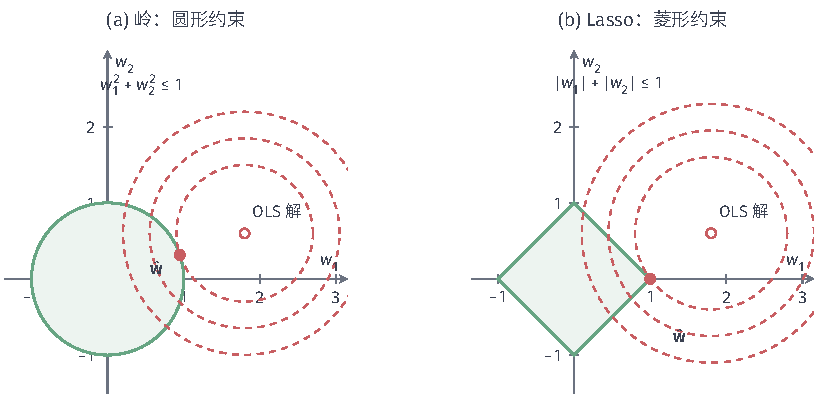
\includegraphics[width=\linewidth]{figures/03-models/01-classic-models/tikz/regression-regularization-geometry/figure.pdf}
  \caption{岭与Lasso的约束几何。构造损失为$J(\bm{w})=\lVert\bm{w}-(1.8,0.6)^{\top}\rVert_2^2/2$，虚线为等损失线，浅色区域为可行域，空心点为OLS解，实心点为约束最优解。左图解为$(1.8,0.6)^{\top}/\sqrt{3.6}$，右图解为$(1,0)^{\top}$。两图都取单位约束半径以比较形状，不表示相同的惩罚强度；Lasso也并非总在尖点取到最优解。}
  \label{fig:regression-regularization-geometry}
\end{figure*}

岭惩罚并不把所有原始坐标按同一比例缩小，下面的谱分解会给出一般设计下的收缩方向。惩罚的概率解释同样依赖归一化：高斯似然下，高斯先验对应二次惩罚，各系数独立的拉普拉斯先验（Laplace prior）对应一范数惩罚，但先验尺度与$\lambda$的对应关系还包含$n$和噪声方差。

\subsubsection{参数学习}
\label{sec:regression-regularization-learning}

岭目标的梯度为零给出
\begin{equation}
  \widehat{\bm{w}}_{\lambda}
  =(\bm{X}^{\top}\bm{X}+n\lambda\bm{I})^{-1}\bm{X}^{\top}\bm{y},
  \qquad\lambda>0.
  \label{eq:regression-ridge-solution}
\end{equation}
任意非零$\bm{v}$满足$\bm{v}^{\top}(\bm{X}^{\top}\bm{X}+n\lambda\bm{I})\bm{v}=\lVert\bm{X}\bm{v}\rVert_2^2+n\lambda\lVert\bm{v}\rVert_2^2>0$，所以即使设计秩亏，斜率解也唯一。若$\gamma_{\max},\gamma_{\min}$是$\bm{X}^{\top}\bm{X}$的极端特征值，正则化后该矩阵的条件数为$(\gamma_{\max}+n\lambda)/(\gamma_{\min}+n\lambda)$；比较对象是正规方程矩阵，而非$\bm{X}$本身的条件数。

取$\bm{X}=\bm{U}_r\bm{D}_r\bm{V}_r^{\top}$，正奇异值为$s_j$，则
\begin{equation}
  \bm{X}\widehat{\bm{w}}_{\lambda}
  =\sum_{j=1}^{r}\frac{s_j^2}{s_j^2+n\lambda}
       \bm{u}_j\bm{u}_j^{\top}\bm{y}.
  \label{eq:regression-ridge-spectral}
\end{equation}
OLS保留列空间中的全部投影，岭回归则按$s_j^2/(s_j^2+n\lambda)$保留各方向，小奇异值方向受到更强收缩。这是稳定性改善的来源，也说明惩罚会同时压低这些方向上的真实信号。

Lasso的目标记为$F(\bm{w})$。由于$\lambda>0$时$F(\bm{w})\geq\lambda\lVert\bm{w}\rVert_1$，连续目标至少取得一个最小值；参数解未必唯一。要理解零系数为何可能最优，可以先固定其他坐标。令$\bm{r}_{-j}=\bm{y}-\sum_{k\ne j}\bm{X}_{:,k}w_k$，$a_j=\lVert\bm{X}_{:,j}\rVert_2^2/n$、$c_j=\bm{X}_{:,j}^{\top}\bm{r}_{-j}/n$，略去常数后的单坐标目标为
\[
  q_j(w_j)=\frac{a_j}{2}w_j^2-c_jw_j+\lambda|w_j|.
\]
在零点左侧，绝对值项的斜率为$-\lambda$；右侧则为$\lambda$。因此零点的左右导数分别为
\[
  q'_{j,-}(0)=-c_j-\lambda,\qquad
  q'_{j,+}(0)=-c_j+\lambda.
\]
这个目标是凸函数，零点最优恰好要求左导数不大于零、右导数不小于零，即$|c_j|\leq\lambda$。此时无论向哪一侧离开零点，目标都不会降低；损失项在零点的导数$-c_j$却不必为零。

为了统一写出光滑点与尖点的条件，引入\term{次梯度}（subgradient）。对一维凸函数$f$，若斜率$s$满足$f(v)\geq f(u)+s(v-u)$对所有$v$成立，它就是$f$在$u$处的一个次梯度：经过该点、斜率为$s$的直线始终位于函数图像下方。所有这样的斜率组成次梯度集合$\partial f(u)$；可导时集合只有导数一个元素，而$|u|$在零点允许$[-1,1]$中的全部斜率。凸函数的最优性因而可统一表为$0\in\partial f(u)$。对Lasso，损失梯度加上惩罚次梯度为零，得到充要最优性条件
\begin{equation}
  \frac{\bm{X}^{\top}(\bm{y}-\bm{X}\widehat{\bm{w}})}{n}
  =\lambda\bm{z},\qquad
  z_j\in
  \begin{cases}
    \{\operatorname{sign}(\widehat w_j)\},&\widehat w_j\ne0,\\
    [-1,1],&\widehat w_j=0.
  \end{cases}
  \label{eq:regression-lasso-kkt}
\end{equation}
其中非零坐标对应的绝对值导数为符号函数，零坐标则允许整个区间来抵消损失梯度。沿用上述$a_j,c_j$，在正、负半轴求导，并在零点检验$|c_j|\leq\lambda$，得到坐标更新
\begin{equation}
  w_j\leftarrow\frac{\mathcal{S}_{\lambda}(c_j)}{a_j},
  \qquad
  \mathcal{S}_{\lambda}(c)=\operatorname{sign}(c)(|c|-\lambda)_+.
  \label{eq:regression-soft-threshold}
\end{equation}
这里$a_j>0$，零列直接取零系数。\term{软阈值}（soft thresholding）把阈值内的量置零，将其余量向零移动$\lambda$。例如正交标准化设计下，OLS系数$(0.12,1.40)$在$\lambda=0.20$时变为$(0,1.20)$；相关设计则需反复更新部分残差，不能直接阈值化OLS系数。循环坐标下降可用式\eqref{eq:regression-lasso-kkt}的违反程度作为停止依据。

弹性网的坐标更新为$\mathcal{S}_{\lambda_1}(c_j)/(a_j+\lambda_2)$。组惩罚则可用近端梯度：先令$\bm{v}=\bm{w}-t\bm{X}^{\top}(\bm{X}\bm{w}-\bm{y})/n$，再逐组计算
\begin{equation}
  \bm{w}_{A_g}^{+}
  =
  \begin{cases}
    \bm{0},&\lVert\bm{v}_{A_g}\rVert_2\leq t\lambda\omega_g,\\
    \left(1-\dfrac{t\lambda\omega_g}{\lVert\bm{v}_{A_g}\rVert_2}\right)
      \bm{v}_{A_g},&\text{其他情形}.
  \end{cases}
  \label{eq:regression-group-prox}
\end{equation}
该式求解的是$\min_{\bm{u}}\lVert\bm{u}-\bm{v}_{A_g}\rVert_2^2/2+t\lambda\omega_g\lVert\bm{u}\rVert_2$：固定$\lVert\bm{u}\rVert_2$时，同向选择使平方距离最小，剩下的一维非负半轴问题给出径向阈值。它是近端子问题的闭式解，不能不加条件地当作任意设计下的精确块坐标解。对非零设计，取$0<t\leq1/\lVert\bm{X}^{\top}\bm{X}/n\rVert_2$可保证凸近端梯度法的目标收敛性质。

沿$\lambda$网格使用前一个解热启动，可以减少重复计算。LARS的Lasso修正版利用分段线性路径求解一范数惩罚问题，但这一性质不直接推广到一般Group Lasso。超参数通常由交叉验证选择；中心化、标准化与变量选择都必须在每个训练折内完成。不同软件对平方损失和惩罚的系数约定不同，不能只按参数名复制同一数值\scite{hastie2009}

\subsubsection{理论分析}
\label{sec:regression-regularization-theory}

惩罚项一方面改变固定训练设计上的优化问题，另一方面改变估计量的偏差、方差和支持恢复。下面先给出确定性的全局最优性，再条件于固定设计比较参数均方误差，并在附加噪声分布下讨论符号恢复的高概率事件。参数收缩或支持恢复仍不能推出任意测试分布上的预测优势，更不能推出因果效应。

\paragraph{收敛性分析}
凸性保证满足最优性条件的点是全局最优点，但迭代算法仍需合适的步长。岭回归在$\lambda>0$时具有正定Hessian，梯度下降可按前述谱条件选择步长；Lasso与组Lasso的近端更新则需同时处理光滑损失和非光滑惩罚。目标值收敛与参数解唯一是不同性质：岭与含正二次惩罚的弹性网有唯一斜率解，Lasso的唯一性还取决于设计和活跃坐标。

\paragraph{泛化分析}
经验目标达到最小，并不保证未来预测误差也最小。正则化通过偏差与方差的变化影响统计误差。岭回归的一个精确结论是：在固定设计与真参数下，足够小的正收缩可以降低参数均方误差。

\begin{figure}[htbp]
  \centering
  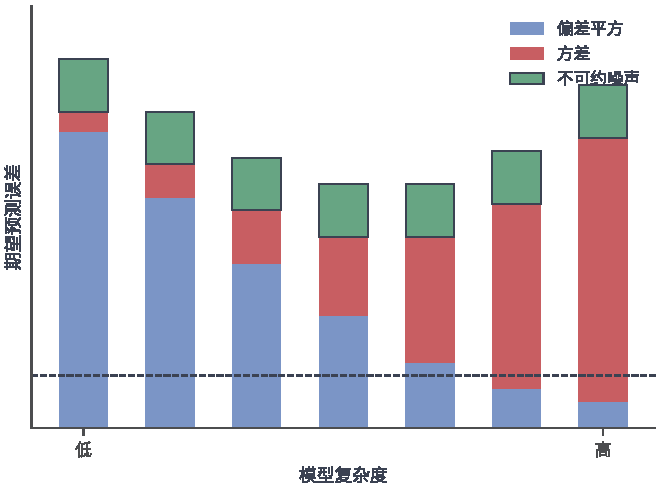
\includegraphics[width=\linewidth]{figures/03-models/01-classic-models/matplotlib/regression-bias-variance-noise/figure.pdf}
  \caption{模型复杂度变化时的偏差—方差—噪声分解示意。柱高是教学构造的相对量，不来自实验：复杂度增加时偏差平方下降、估计方差上升，不可约噪声保持不变。总误差由三部分共同决定，因此“模型更复杂”与“误差更小”都不是无条件结论。}
  \label{fig:regression-bias-variance-noise}
\end{figure}

\Needspace{8\baselineskip}
\begin{theorem}[小幅岭收缩的参数均方误差]
  \label{thm:regression-ridge-mse}
  设$\bm{y}=\bm{X}\bm{w}_{\star}+\bm{\varepsilon}$，固定设计$\bm{X}$列满秩，参数维数至少为$1$，噪声均值为零、协方差为$\sigma^2\bm{I}$，且$\sigma^2>0$。则存在$\lambda_0>0$，使所有$0<\lambda<\lambda_0$的岭估计参数均方误差严格小于OLS。
\end{theorem}

\begin{proof}
令$a=n\lambda$，将$\bm{X}^{\top}\bm{X}$正交对角化，特征值为$\gamma_j>0$，真参数在相应方向上的坐标为$\theta_j$。岭估计在第$j$个方向上的偏差为$-a\theta_j/(\gamma_j+a)$，方差为$\sigma^2\gamma_j/(\gamma_j+a)^2$。正交变换保持欧氏范数，故参数均方误差为
\[
  M(a)=\sum_j\frac{a^2\theta_j^2+\sigma^2\gamma_j}{(\gamma_j+a)^2}.
\]
函数在$a=0$附近可微，且$M'(0)=-2\sigma^2\sum_j\gamma_j^{-2}<0$。导数定义保证存在$a_0>0$，使所有$0<a<a_0$满足$M(a)<M(0)$。取$\lambda_0=a_0/n$即可。
\end{proof}

中心化响应会使噪声协方差变成$\sigma^2(\bm{I}-\bm{1}\bm{1}^{\top}/n)$，但中心化设计满足$\bm{X}^{\top}\bm{1}=\bm{0}$，所以斜率方向上的上述计算仍成立。定理没有给出不依赖未知真参数的最优$\lambda$，也不意味着任意收缩都改善任意测试分布的预测风险。

Lasso能否认出真实非零变量，则是更强的问题。仅有稀疏性还不够：无关变量若可由相关变量近似替代，就难以判定贡献应归给谁。\term{不可表示条件}（irrepresentable condition）限制这种替代关系；符号恢复还需要噪声和最小信号条件\scite{zhao2006lasso}

\Needspace{18\baselineskip}
\begin{theorem}[Lasso的确定性符号恢复充分条件]
  \label{thm:regression-lasso-recovery}
  设$\bm{y}=\bm{X}\bm{w}_{\star}+\bm{\varepsilon}$，$A=\{j:w_{\star,j}\ne0\}$非空，$\bm{X}_A=\bm{X}_{:,A}$列满秩。记
  \[
    \bm{G}=\bm{X}^{\top}\bm{X}/n,\quad
    \bm{s}=\operatorname{sign}(\bm{w}_{\star,A}),\quad
    \bm{P}_A=\bm{X}_A(\bm{X}_A^{\top}\bm{X}_A)^{-1}\bm{X}_A^{\top},
  \]
  以及$\bm{q}=\bm{G}_{A,A}^{-1}\bm{X}_A^{\top}\bm{\varepsilon}/n$、$\bm{b}=\bm{G}_{A,A}^{-1}\bm{s}$。若$\lambda>0$，且存在$0<\eta\leq1$使
  \begin{align}
    \lVert\bm{G}_{A^c,A}\bm{G}_{A,A}^{-1}\bm{s}\rVert_\infty
      &\leq1-\eta, \label{eq:regression-irrepresentable}\\
    \left\lVert\bm{X}_{A^c}^{\top}(\bm{I}-\bm{P}_A)
                  \bm{\varepsilon}/n\right\rVert_\infty
      &\leq\lambda\eta/2, \label{eq:regression-lasso-noise}\\
    \min_{j\in A}|w_{\star,j}|
      &>\lVert\bm{q}\rVert_\infty+\lambda\lVert\bm{b}\rVert_\infty,
      \label{eq:regression-lasso-beta-min}
  \end{align}
  则Lasso解唯一，且$\operatorname{sign}(\widehat{\bm{w}})=\operatorname{sign}(\bm{w}_{\star})$。$A^c$为空时，前两个条件为空条件。
\end{theorem}

\begin{proof}
构造$\widetilde{\bm{w}}_{A^c}=\bm{0}$、$\widetilde{\bm{w}}_A=\bm{w}_{\star,A}+\bm{q}-\lambda\bm{b}$。最小信号条件保证每个活跃坐标的扰动小于其原绝对值，因此符号仍为$\bm{s}$。残差满足
\[
  \bm{r}=\bm{y}-\bm{X}\widetilde{\bm{w}}
  =(\bm{I}-\bm{P}_A)\bm{\varepsilon}
   +\lambda\bm{X}_A\bm{G}_{A,A}^{-1}\bm{s}.
\]
令$\widetilde{\bm{z}}=\bm{X}^{\top}\bm{r}/(n\lambda)$，则$\widetilde{\bm{z}}_A=\bm{s}$，且
\[
  \widetilde{\bm{z}}_{A^c}
  =\bm{G}_{A^c,A}\bm{G}_{A,A}^{-1}\bm{s}
    +\frac{\bm{X}_{A^c}^{\top}(\bm{I}-\bm{P}_A)
            \bm{\varepsilon}}{n\lambda}.
\]
前两个条件给出$\lVert\widetilde{\bm{z}}_{A^c}\rVert_\infty\leq1-\eta/2<1$。因此$\widetilde{\bm{z}}$是合法次梯度，式\eqref{eq:regression-lasso-kkt}成立，候选解最优。

对任意扰动$\bm{h}$，精确展开目标差并代入平稳条件，得到
\[
  \begin{aligned}
    F(\widetilde{\bm{w}}+\bm{h})-F(\widetilde{\bm{w}})
    ={}&\frac{\lVert\bm{X}\bm{h}\rVert_2^2}{2n}\\
      &+\lambda\bigl(\lVert\widetilde{\bm{w}}+\bm{h}\rVert_1
         -\lVert\widetilde{\bm{w}}\rVert_1
         -\widetilde{\bm{z}}^{\top}\bm{h}\bigr).
  \end{aligned}
\]
活跃坐标的括号贡献由次梯度不等式非负；非活跃坐标的贡献至少为$(\eta/2)|h_j|$。若扰动后仍最优，必有$\bm{h}_{A^c}=\bm{0}$与$\bm{X}\bm{h}=\bm{0}$，故$\bm{X}_A\bm{h}_A=\bm{0}$。活跃设计满列秩进一步推出$\bm{h}_A=\bm{0}$，唯一性得证。
\end{proof}

这个命题直接约束一份数据中的噪声向量，不需要高斯假设。要得到高概率恢复，还须对这些约束的概率作估计。例如在固定设计、独立高斯噪声且$\lVert\bm{X}_{:,j}\rVert_2\leq\sqrt n$下，并合界给出
\[
  \mathbb{P}\!\left(
    \lVert\bm{X}_{A^c}^{\top}(\bm{I}-\bm{P}_A)
       \bm{\varepsilon}/n\rVert_\infty>\lambda\eta/2
  \right)
  \leq2|A^c|\exp\!\left(-\frac{n\lambda^2\eta^2}{8\sigma^2}\right).
\]
活跃坐标上的$\bm{q}$还须另外控制，不能只凭这个尾界完成恢复结论。预测准确、支持集恢复和因果解释也不同：两个相关特征的替换可能几乎不影响预测，却改变所选变量；非零预测系数本身不能证明干预效应。

\subsubsection{支持相关特征的分组稳定（Elastic Net）}
\label{sec:regression-elastic-net}

弹性网中的$\lambda_2>0$使整个目标严格凸，即使设计秩亏也有唯一参数解。若两列完全相同，交换相应系数不改变目标，唯一性便要求两个系数相等。二次惩罚由此排除了完全相同特征之间任意分摊系数的歧义。

对两个非零且同号的系数，把各自的最优性条件相减，可得
\[
  \lambda_2|\widehat w_j-\widehat w_k|
  \leq\frac{\lVert\bm{X}_{:,j}-\bm{X}_{:,k}\rVert_2
                  \lVert\bm{y}-\bm{X}\widehat{\bm{w}}\rVert_2}{n}.
\]
因此在相同尺度下，两列越接近，其同号估计越接近。这个界以非零同号为条件，不保证任何相关变量组都被选中。实际选择$\alpha,\lambda$时，仍应根据预测或变量选择的目标验证稳定性。

\subsubsection{支持结构化稀疏（Group Lasso）}
\label{sec:regression-group-lasso}

一个类别变量的多个指示变量，或一个连续变量的整组样条基，常需要作为整体评价。组Lasso把这样的先验分组写进惩罚；在非零组上，惩罚的梯度方向是$\bm{w}_{A_g}/\lVert\bm{w}_{A_g}\rVert_2$，零组处的次梯度则是单位球。组内残差相关向量未超过$\lambda\omega_g$时，整组可以保持为零。

权重$\sqrt{|A_g|}$能补偿组大小的一部分影响，但并不消除组内相关性或量纲差异。若还希望在保留组内继续选择坐标，可使用\term{稀疏组Lasso}（sparse group Lasso），即在组惩罚之外再加$\lambda_1\lVert\bm{w}\rVert_1$。这同时约束组与坐标两个层次；选择一致性仍需要适当设计、信号强度及正则化条件，不能仅由“真实参数有组结构”推出。

\subsubsection{小结}
\label{sec:regression-regularization-summary}

岭、Lasso、弹性网与组Lasso分别强调连续收缩、坐标稀疏、相关系数稳定性和组稀疏。它们共享凸损失加惩罚的框架，但并不共享所有路径算法或恢复定理。进一步的相关工作还包括自适应加权的Adaptive Lasso、惩罚相邻系数差的Fused Lasso，以及对大系数减弱收缩的SCAD和MCP非凸惩罚。“Oracle性质”指在特定渐近条件下达到仿佛已知真支持集的估计行为，不是这些方法在任意数据上的保证；非凸惩罚还带来局部最优的计算问题\scite{hastie2009}

处理共线性的另一条路线是先降维再回归。\term{主成分回归}（principal component regression, PCR）保留若干主成分，在这些正交方向上拟合，等价于对选中方向完全保留、对其余方向硬截断。第\ref{sec:dim-pca}节从无监督表示的角度推导主成分分析（PCA）：PCA与PCR共享由输入方差确定的主成分基，但PCA按方差保留与重构误差评价表示，PCR还要用响应检验这些成分是否有利于预测。与式\eqref{eq:regression-ridge-spectral}的连续收缩相比，PCR的取舍更直接，但输入方差小不意味着对响应不重要。\term{偏最小二乘回归}（partial least squares regression, PLS）在构造成分时同时利用输入与响应的关系，因而属于监督降维；它有不同的具体算法，不能笼统理解为收缩因子必在$0$和$1$之间的岭回归。成分数同样需要在训练折内选择。

\subsection{分位数回归（Quantile Regression）}
\label{sec:regression-quantiles}

预算制定者关心的是实际支出超过预算的概率，单个条件均值无法回答这个问题。\term{分位数回归}（quantile regression）用非对称残差损失估计给定输入后的指定分位数；例如$0.9$分位数提供一个使响应至少有$90\%$概率不超过它的条件阈值。Koenker与Bassett在1978年系统提出回归分位数，将回归目标从条件均值扩展到条件分布的不同位置。这一区分源于决策目标，无需先假定误差对称或同方差\scite{koenker1978quantiles}

\subsubsection{模型结构}

给定$0<\tau<1$，定义\term{分位数损失}（pinball loss）
\begin{equation}
  \rho_\tau(r)=
  \begin{cases}
    \tau r,&r\geq0,\\
    (1-\tau)(-r),&r<0.
  \end{cases}
  \label{eq:regression-pinball}
\end{equation}
残差仍取$r=y-\widehat y$，所以较大的$\tau$更重地惩罚低估。线性分位数回归最小化$\sum_i\rho_\tau(y_i-\bm{\phi}(\bm{x}_i)^{\top}\bm{w})$。这一形式为何对应分位数，可以直接证明。

\Needspace{8\baselineskip}
\begin{theorem}[分位数损失的总体最优解]
  \label{thm:regression-quantile}
  若$\mathbb{E}|Y|<\infty$，分布函数为$F_Y$，则$Q(a)=\mathbb{E}[\rho_\tau(Y-a)]$的全部最小化点恰好满足
  \[
    F_Y(a-)\leq\tau\leq F_Y(a),
    \qquad F_Y(a-)=\mathbb{P}(Y<a).
  \]
\end{theorem}

\begin{proof}
对固定$Y$，损失关于$a$凸，斜率绝对值不超过$1$。有界收敛允许单侧差商与期望交换。当$Y<a$时斜率为$1-\tau$，当$Y>a$时为$-\tau$；在$Y=a$处左、右导数分别取这两个值中的$-\tau$与$1-\tau$。故
\[
  Q'_-(a)=F_Y(a-)-\tau,\qquad Q'_+(a)=F_Y(a)-\tau.
\]
凸函数在$a$处最小当且仅当$Q'_-(a)\leq0\leq Q'_+(a)$。分布函数从$0$增长到$1$，保证这样的点存在。
\end{proof}

将分布换成给定输入的条件分布，便得到条件分位数；换成经验分布，便得到样本分位数。$\tau=1/2$时损失为$|r|/2$，对应中位数。分布存在原子或平台时最优点可能不唯一，因此不能一律写成$F_Y(a)=\tau$。在线性模型受到限制时，只有正确指定等条件下才能精确表示真实条件分位数，一般得到该函数类中的最佳损失逼近。

\subsubsection{参数学习}

引入非负正、负残差$\bm{u},\bm{v}\in\mathbb{R}^{n}$，可将目标写成线性规划
\begin{equation}
  \begin{aligned}
    \min_{\bm{w},\bm{u},\bm{v}}\quad&
      \tau\bm{1}^{\top}\bm{u}+(1-\tau)\bm{1}^{\top}\bm{v},\\
    \text{满足}\quad&
      \bm{y}-\bm{X}\bm{w}=\bm{u}-\bm{v},
      \quad\bm{u}\geq\bm{0},\ \bm{v}\geq\bm{0}.
  \end{aligned}
  \label{eq:regression-quantile-lp}
\end{equation}
若某个$u_i,v_i$同时为正，同时减小二者保持约束不变且严格降低目标，因此最优时二者不会同时为正，线性规划与原损失等价。可采用单纯形法、内点法或适合数据规模的非光滑凸优化算法；非光滑不意味着只能使用线性规划。

高维时可在平均分位数损失之外增加$\lambda\lVert\bm{w}\rVert_1$，通过把系数也拆为正负部分继续写成线性规划。多个$\tau$可以分别拟合，也可以联合加入顺序约束；超参数评价应使用对应的分位数损失，而不是仅凭平方误差判断。

\subsubsection{小结}

分位数回归把预测从条件均值扩展到分布中的指定位置，多个分位数有助于描述分布形状，但有限网格不等于完整条件分布。独立拟合可能出现较高分位数反而更低的分位数交叉，联合约束需说明在哪些输入上生效。线性尾部损失降低了大残差的边际作用，却不自动抵御高杠杆点；极端分位数仍需要足够尾部数据。预测区间由分位数组成后，其覆盖率也需要单独评价。

\subsection{支持向量回归（SVR）}
\label{sec:regression-svr}

另一种误差评价允许小偏差不计损失，只惩罚超出容忍范围的部分。\term{支持向量回归}（support vector regression, SVR）将这种损失与二次正则化结合，得到一个由训练样本加权表示的预测函数。部分样本的权重可以为零，核化以后只需保留非零权重对应的样本来计算预测。这是样本展开的稀疏性，与Lasso选择输入变量的稀疏性不同\scite{smola2004svr}

\subsubsection{模型结构}

设$\epsilon\geq0$，定义\term{$\epsilon$不敏感损失}（$\epsilon$-insensitive loss）为$L_\epsilon(r)=(|r|-\epsilon)_+$。它把$\pm\epsilon$之间的残差视为可容忍误差，超出部分线性计入损失。线性SVR单独保留不受惩罚的截距$b$，目标为
\begin{equation}
  \min_{\bm{w},b}\;
    \frac12\lVert\bm{w}\rVert_2^2+
    C\sum_{i=1}^{n}L_\epsilon(y_i-\bm{w}^{\top}\bm{x}_i-b),
    \qquad C>0.
  \label{eq:regression-svr-objective}
\end{equation}
除以$nC$，可知它与“平均损失$+\lambda\lVert\bm{w}\rVert_2^2/2$”在$\lambda=1/(nC)$时等价。$C$越大，训练误差在目标中的相对权重越大；$\epsilon$则具有响应的单位，规定不计损失的范围。

为推导对偶问题，引入$\xi_i^+,\xi_i^-\geq0$，分别表示两个方向超出容忍带的量。等价约束形式为
\begin{equation}
  \begin{aligned}
    \min_{\bm{w},b,\bm{\xi}^+,\bm{\xi}^-}\quad&
       \tfrac12\lVert\bm{w}\rVert_2^2+C\sum_i(\xi_i^++\xi_i^-),\\
    \text{满足}\quad&
       y_i-\bm{w}^{\top}\bm{x}_i-b\leq\epsilon+\xi_i^+,\\
      &\bm{w}^{\top}\bm{x}_i+b-y_i\leq\epsilon+\xi_i^-,\\
      &\xi_i^+,\xi_i^-\geq0,\qquad i=1,\ldots,n.
  \end{aligned}
  \label{eq:regression-svr-primal}
\end{equation}
固定预测时，由$C>0$可知最优松弛量恰为超出带宽的部分。$\epsilon=0$对应带二次惩罚的绝对损失回归。对固定有限数据，若$\epsilon\geq(\max_i y_i-\min_i y_i)/2$，则$\bm{w}=\bm{0}$和某个常数$b$已能使全部样本进入容忍带，目标取得零值。截距在此时可能不唯一。

\subsubsection{参数学习}

原问题是在可行参数中寻找最小目标值，为什么下面会出现一个最大化问题？把各不等式写成“左边不大于零”，分别乘以非负的拉格朗日乘子并加到目标中，就得到拉格朗日函数。在任一可行点，这些附加项都不大于零；固定乘子，再对全部原始变量取下确界，便得到原问题最优值的一个下界。选择乘子把这个下界尽量抬高，就是\term{对偶}（dual）最大化。乘子在这里用于构造下界；若最佳下界等于原问题的最小值，就称为\term{强对偶}（strong duality）。

下面用凸优化条件判断这一对应何时成立。Slater条件要求在满足等式约束的同时存在严格可行的不等式点，它在当前凸问题中用于建立强对偶；KKT条件把原始可行性、对偶可行性、驻点条件和互补松弛放在同一组方程中，其中互补松弛要求乘子与对应约束余量的乘积为零。在凸问题满足Slater条件时，KKT条件对最优性既必要又充分；分类SVM中的对应条件见式\eqref{eq:classification-svm-hard-kkt}。

为前两组约束引入乘子$\alpha_i^+,\alpha_i^-\geq0$，为松弛量非负约束引入$\mu_i^+,\mu_i^-\geq0$。令$r_i=y_i-\bm{w}^{\top}\bm{x}_i-b$，拉格朗日函数为
\[
  \begin{aligned}
    \mathcal{L}={}&\tfrac12\lVert\bm{w}\rVert_2^2
       +C\sum_i(\xi_i^++\xi_i^-)
       +\sum_i\alpha_i^+(r_i-\epsilon-\xi_i^+)\\
       &+\sum_i\alpha_i^-(-r_i-\epsilon-\xi_i^-)
       -\sum_i(\mu_i^+\xi_i^++\mu_i^-\xi_i^-).
  \end{aligned}
\]
分别对$\bm{w},b,\xi_i^\pm$求导，得到
\[
  \bm{w}=\sum_i(\alpha_i^+-\alpha_i^-)\bm{x}_i,\qquad
  \sum_i(\alpha_i^+-\alpha_i^-)=0,\qquad
  C-\alpha_i^\pm-\mu_i^\pm=0.
\]
最后一式给出$0\leq\alpha_i^\pm\leq C$。记$\beta_i=\alpha_i^+-\alpha_i^-$，消去原始变量后，对偶问题为
\begin{equation}
  \begin{aligned}
    \max_{\bm{\alpha}^+,\bm{\alpha}^-}\quad&
       -\tfrac12\sum_{i,j}\beta_i\beta_j\bm{x}_i^{\top}\bm{x}_j
       -\epsilon\sum_i(\alpha_i^++\alpha_i^-)
       +\sum_i y_i\beta_i,\\
    \text{满足}\quad&
       \sum_i\beta_i=0,\qquad 0\leq\alpha_i^\pm\leq C.
  \end{aligned}
  \label{eq:regression-svr-dual}
\end{equation}
原始问题凸，选择足够大的正松弛量即可严格满足不等式，因此满足Slater条件，强对偶成立。对偶是带盒约束与一个线性等式约束的凸二次规划的最大化写法，可通过分解算法逐步更新少量变量；每次更新应保持等式约束，并以最优性残差作为停止依据。

得到乘子后，若$0<\alpha_i^+<C$，互补松弛给出$r_i=\epsilon$，所以$b=y_i-\bm{w}^{\top}\bm{x}_i-\epsilon$；若$0<\alpha_i^-<C$，则$b=y_i-\bm{w}^{\top}\bm{x}_i+\epsilon$。可对多个此类样本的截距估计取平均以减小数值误差。若没有内点乘子，应根据全部KKT不等式求可行截距区间，不能假设总能找到一个严格介于$0$与$C$之间的乘子。

\subsubsection{理论分析}

SVR的对偶结构能够回答固定训练集上的凸最优性，却不能直接回答独立新样本上的预测风险。前者可由对偶间隙和KKT残差作确定性判断；后者还须给出抽样制度、函数类与响应尾部条件。因而，支持向量较少或优化误差较小不能推出分布无关的泛化保证。

\paragraph{收敛性分析}
SVR的原始问题是凸优化问题，前述强对偶与KKT条件给出了全局最优性的判据。数值求解时，可以用原始可行解与对偶可行解的目标差距控制尚未消除的优化误差；具体迭代的收敛速度仍取决于求解器、设计与核矩阵。

支持向量与残差位置的关系必须区分带内、带外和边界三个情况。边界上的约束虽然取等号，乘子仍然可以为零。

\Needspace{16\baselineskip}
\begin{theorem}[SVR的样本系数与残差]
  \label{thm:regression-svr-support}
  设$\epsilon>0$，在任意一组原始与对偶最优解处记$r_i=y_i-\bm{w}^{\top}\bm{x}_i-b$、$\beta_i=\alpha_i^+-\alpha_i^-$。则
  \[
    \begin{array}{c|c}
      \text{残差位置}&\text{对偶乘子}\\ \hline
      |r_i|<\epsilon&\alpha_i^+=\alpha_i^-=0\\
      r_i>\epsilon&\alpha_i^+=C,\ \alpha_i^-=0\\
      r_i<-\epsilon&\alpha_i^+=0,\ \alpha_i^-=C\\
      r_i=\epsilon&\alpha_i^+\in[0,C],\ \alpha_i^-=0\\
      r_i=-\epsilon&\alpha_i^+=0,\ \alpha_i^-\in[0,C]
    \end{array}
  \]
  因而$\beta_i\ne0$蕴含$|r_i|\geq\epsilon$，反向蕴含在边界处不成立。
\end{theorem}

\begin{proof}
最优松弛量为$\xi_i^+=(r_i-\epsilon)_+$、$\xi_i^-=(-r_i-\epsilon)_+$。KKT互补松弛条件为
\[
  \alpha_i^+(\epsilon+\xi_i^+-r_i)=0,\qquad
  \alpha_i^-(\epsilon+\xi_i^-+r_i)=0,\qquad
  (C-\alpha_i^\pm)\xi_i^\pm=0.
\]
严格带内时两个残差约束都松弛，故两个乘子均为零。若$r_i>\epsilon$，则$\xi_i^+>0$迫使$\alpha_i^+=C$，另一个残差约束严格松弛，故$\alpha_i^-=0$；负向带外同理。若$r_i=\epsilon$，正向松弛量为零，其乘子仅受盒约束限制；由于$\epsilon>0$，负向残差约束严格松弛，故$\alpha_i^-=0$。另一侧边界同理。
\end{proof}

一个反例足以排除边界处的“当且仅当”：取单个样本、$\bm{x}_1=\bm{0}$，令$\bm{w}=\bm{0}$、$b=y_1-\epsilon$，则$r_1=\epsilon$，原始目标为零；两个乘子均为零也满足对偶最优性。这个边界样本的系数为零。$\epsilon=0$时两个边界重合，零残差处两类乘子可能同时非零，必须单独处理，不能沿用上表的两行边界结论。

\paragraph{泛化分析}
稀疏性由实际最优解决定，支持向量数并不保证随着$\epsilon$严格单调下降；改变$\epsilon$也会改变整条预测函数。评价泛化还需控制函数类及数据分布，例如核对角线、参数范数、截距或响应尾部。仅凭支持向量少，不能推出测试误差小。有限步数的优化误差与由有限样本造成的统计误差，也应分别评价。

\subsubsection{支持非线性回归（核 SVR）}
\label{sec:regression-kernel-svr}

使用第\ref{sec:classic-overview-kernel-trick}节的正定核$K$，把式\eqref{eq:regression-svr-dual}中的$\bm{x}_i^{\top}\bm{x}_j$换为$K(\bm{x}_i,\bm{x}_j)$，便得到特征空间中的同一个SVR对偶问题。预测为
\begin{equation}
  f(\bm{x})=\sum_{i=1}^{n}\beta_i K(\bm{x}_i,\bm{x})+b.
  \label{eq:regression-kernel-svr-prediction}
\end{equation}
核函数及其合法性见第\ref{sec:classic-overview-kernel-validity}节与第\ref{sec:classic-overview-common-kernels}节。此处新增的是$\epsilon$不敏感响应损失与系数约束；分类SVM使用的间隔损失不会因此变成回归目标。

核SVR沿用相同的对偶结构，但计算规模从显式特征维数转向训练样本数。核矩阵若完整保存需要$O(n^2)$空间，采用缓存可以降低内存占用；训练时间还依赖求解器、精度及数据条件。预测需要约$n_{\mathrm{SV}}$次核计算，其中$n_{\mathrm{SV}}$为非零展开系数的样本数。线性核则可预先合并$\bm{w}$，使预测成本恢复为$O(d)$。

\subsubsection{小结}

SVR在固定容忍带下折中残差代价与函数范数，核化使这种折中作用于非线性函数类。它不直接针对任意$\tau$的条件分位数，也不由损失形式自动产生完整预测分布。$\nu$-SVR通过另一个参数控制与误差比例、支持向量比例有关的约束，具体比例结论有相应条件；最小二乘SVR把损失换为平方形式，与核岭回归密切相关，但是否惩罚截距必须一致后才能判断等价。核选择与$C,\epsilon$调参共同影响结果，不能按一个固定样本量门槛判断方法是否适用。

\subsection{广义线性模型（GLM）}
\label{sec:regression-glm}

预测每天的交易次数时，均值必须非负；预测交易是否成功时，均值是$[0,1]$中的概率。平方损失可以用于这些响应，但无约束线性预测不自动满足取值范围，也没有规定均值与方差的关系。\term{广义线性模型}（generalized linear model, GLM）把响应分布、均值和线性预测器连接起来。Nelder与Wedderburn在1972年给出这一统一框架，使高斯、二项和Poisson等响应可以沿同一条似然与加权最小二乘路线处理；扩展的关键是响应分布与链接，而不只是增加多项式特征\scite{nelder1972glm}

\subsubsection{模型结构}

条件于输入，假设响应相互独立，密度或概率质量函数具有指数族形式
\begin{equation}
  p(y_i\mid\theta_i,\varphi)
  =\exp\!\left\{
    \frac{y_i\theta_i-b(\theta_i)}{a(\varphi)}
    +c(y_i,\varphi)\right\},\qquad a(\varphi)>0.
  \label{eq:regression-exponential-family}
\end{equation}
$\theta_i$是自然参数，$\varphi$是离散度参数或尺度参数；此处为便于推导，所有观测使用相同的$a(\varphi)$。函数$a,b,c$的形式由选定的分布族确定，并不作为三个未知函数一起学习。例如，均值为$\mu_i>0$的Poisson分布可写成
\[
  p(y_i\mid\mu_i)
  =\frac{\mu_i^{y_i}e^{-\mu_i}}{y_i!}
  =\exp\{y_i\log\mu_i-\mu_i-\log(y_i!)\}.
\]
逐项对照式\eqref{eq:regression-exponential-family}，可得$\theta_i=\log\mu_i$、$b(\theta_i)=e^{\theta_i}$、$a(\varphi)=1$、$c(y_i,\varphi)=-\log(y_i!)$。这里没有额外待估的离散度参数，自然参数也不是均值本身。

一般情形下，假定支持集不随$\theta_i$改变，并允许交换积分（离散情形为求和）与微分。密度积分为$1$，对$\theta_i$求导得到$\mathbb{E}[Y_i-b'(\theta_i)]=0$；再求一次导数得到
\[
  \mathbb{E}\!\left[
    \frac{(Y_i-b'(\theta_i))^2}{a(\varphi)^2}
      -\frac{b''(\theta_i)}{a(\varphi)}\right]=0.
\]
因此均值与方差为
\begin{equation}
  \mu_i=b'(\theta_i),\qquad
  \operatorname{Var}(Y_i\mid\bm{x}_i)
  =a(\varphi)b''(\theta_i)=a(\varphi)V(\mu_i).
  \label{eq:regression-glm-moments}
\end{equation}
函数$V$描述方差怎样随均值变化。GLM再引入线性预测器$\eta_i=\bm{\phi}(\bm{x}_i)^{\top}\bm{w}$与\term{链接函数}（link function）$g$，令$g(\mu_i)=\eta_i$。链接作用于条件均值，而不是把每个观测$y_i$变换后做OLS。若$\eta_i=\theta_i$，称为规范链接。

表\ref{tab:regression-glm}列出三种基本组合。伯努利模型的均值就是成功概率，因此logistic回归既可作为概率回归理解，也可在给定决策阈值后用于分类。第\ref{sec:classification-logistic}节沿用伯努利似然、logit链接与IRLS计算，但把重点转向类别标签的概率、决策阈值与校准；本节则借这一特例说明GLM中响应分布、链接和均值方差关系的共同结构。Poisson模型采用对数链接，使$\mu_i=\exp(\eta_i)>0$；响应是整数，条件均值却不必为整数。

\begin{table}[htbp]
  \centering
  \begin{tabular}{llll}
    \toprule
    响应模型 & $b(\theta)$ & 规范链接$g(\mu)$ & $V(\mu)$\\
    \midrule
    高斯 & $\theta^2/2$ & $\mu$ & $1$\\
    伯努利 & $\log(1+e^\theta)$ & $\log\frac{\mu}{1-\mu}$ & $\mu(1-\mu)$\\
    Poisson & $e^\theta$ & $\log\mu$ & $\mu$\\
    \bottomrule
  \end{tabular}
  \caption{GLM的三个常用特例。高斯模型的$a(\varphi)=\sigma^2$，后两者的$a(\varphi)=1$。链接保证均值范围，分布假设进一步规定条件方差。}
  \label{tab:regression-glm}
\end{table}

二项分布可处理已知试验次数下的成功数；Gamma模型可处理正连续响应。链接选择并不唯一，必须同时满足自然参数域和均值域的要求。Poisson的均值方差相等也可能与数据不符，过度离散、零膨胀或观测相关性需要额外建模，不能靠对数链接本身解决。

\subsubsection{参数学习}

记$\bm{z}_i=\bm{\phi}(\bm{x}_i)$，设计矩阵第$i$行为$\bm{z}_i^{\top}$，暂将$\varphi$视为已知。由$d\mu_i/d\theta_i=V(\mu_i)$及$d\eta_i/d\mu_i=g'(\mu_i)$，对数似然的得分为
\begin{equation}
  \bm{U}(\bm{w})
  =\sum_i\frac{y_i-\mu_i}
    {a(\varphi)V(\mu_i)g'(\mu_i)}\bm{z}_i.
  \label{eq:regression-glm-score}
\end{equation}
在所需导数存在且$g'(\mu_i)\ne0$时，期望负Hessian即Fisher信息$\bm{X}^{\top}\bm{W}\bm{X}$，其中
\[
  W_{i,i}=\frac{1}{a(\varphi)V(\mu_i)[g'(\mu_i)]^2}.
\]
\term{Fisher评分}（Fisher scoring）用这个期望曲率修正当前参数，更新$\bm{w}^{+}=\bm{w}+(\bm{X}^{\top}\bm{W}\bm{X})^{-1}\bm{U}(\bm{w})$。要把它写成加权最小二乘，需要先把响应尺度上的误差换算成线性预测器尺度上的修正。在当前均值附近，链接函数的一阶近似为$g(\mu_i+\Delta\mu)\approx\eta_i+g'(\mu_i)\Delta\mu$；将残差$y_i-\mu_i$作为局部修正信号，便得到\term{工作响应}（working response）
\[
  z_i^{\mathrm{work}}
    =\eta_i+(y_i-\mu_i)g'(\mu_i),
\]
它是本轮局部子问题的目标值，会随当前参数改变，并非把真实标签永久变成$g(y_i)$。固定当前参数时，这个仿射换算后的响应方差为$a(\varphi)V(\mu_i)[g'(\mu_i)]^2$，其倒数正是$W_{i,i}$；换算后方差较大的观测因而权重较小。代入可得$\bm{U}=\bm{X}^{\top}\bm{W}(\bm{z}^{\mathrm{work}}-\bm{X}\bm{w})$，从而
\begin{equation}
  \bm{w}^{+}
  =(\bm{X}^{\top}\bm{W}\bm{X})^{-1}
     \bm{X}^{\top}\bm{W}\bm{z}^{\mathrm{work}}.
  \label{eq:regression-irls}
\end{equation}
这就是\term{迭代重加权最小二乘}（iteratively reweighted least squares, IRLS）：在当前均值附近构造一个加权平方子问题。实际使用分解求解线性方程，检查秩、参数域与似然下降情况，必要时采用阻尼或线搜索。各观测共享的$a(\varphi)$在无惩罚参数更新中可以约去，但在信息矩阵和方差计算中不能遗漏。

规范链接下，$\theta_i=\eta_i$，负对数似然的Hessian为
\[
  \frac{1}{a(\varphi)}
  \bm{X}^{\top}\operatorname{diag}(b''(\eta_i))\bm{X}.
\]
它半正定，因此目标凸；若$b''(\eta_i)>0$且设计列满秩，则有限参数域内严格凸。这时Newton法与Fisher评分具有相同的曲率矩阵，但完整步长不自动保证每次都提高似然，更不能保证有限最优解存在。

\subsubsection{理论分析}
\label{sec:regression-glm-theory}

对GLM，首要边界是固定样本上有限最大似然解是否存在以及数值过程能否求到它；只有在模型正确、维数固定且样本独立同分布时，才进一步讨论估计量的渐近分布。相应结论分别是存在性边界与依分布收敛，不能推出有限样本预测风险，也不能把参数区间直接当作未来响应区间。

\paragraph{收敛性分析}
严格凸性只能保证已经存在的最优解唯一。以无惩罚logistic回归为例，若存在方向$\bm{v}$使类别标签$t_i\in\{-1,1\}$满足$t_i\bm{z}_i^{\top}\bm{v}>0$，则负对数似然$\sum_i\log(1+\exp(-t_i\bm{z}_i^{\top}\bm{w}))$在$\bm{w}=a\bm{v}$、$a\to\infty$时趋于零，却在每个有限参数处严格为正。即使设计满秩，也没有有限最大似然估计。分离、近似分离和病态设计都可能使迭代参数持续增大。

\paragraph{泛化分析}
有限样本估计量的分布可以帮助量化参数及预测的不确定性，但它与优化算法的收敛是不同问题。下面给出渐近正态性的充分条件与证明，将估计一致性和局部曲率控制明确列出；具体GLM还需根据分布、链接和输入矩条件验证它们。

\Needspace{16\baselineskip}
\begin{theorem}[正则GLM估计的渐近正态性]
  \label{thm:regression-glm-asymptotic}
  设观测独立同分布，模型正确指定，参数维数固定，真参数$\bm{w}_{\star}$位于参数域内部。单样本对数似然$\ell_i(\bm{w})$在真参数的某凸邻域二阶连续可微，并满足
  \[
    \mathbb{E}[\nabla\ell_i(\bm{w}_{\star})]=\bm{0},\qquad
    \operatorname{Cov}(\nabla\ell_i(\bm{w}_{\star}))=\bm{I}_{\star}\succ0.
  \]
  假设有限的内部最大似然估计$\widehat{\bm{w}}_n$以趋于$1$的概率存在且一致；对$J_n(\bm{w})=-n^{-1}\sum_i\nabla^2\ell_i(\bm{w})$，在该邻域内有一致依概率收敛$J_n\to J$，其中$J$在$\bm{w}_{\star}$连续且$J(\bm{w}_{\star})=\bm{I}_{\star}$。则
  \[
    \sqrt n(\widehat{\bm{w}}_n-\bm{w}_{\star})
      \xrightarrow{d}\mathcal{N}(\bm{0},\bm{I}_{\star}^{-1}).
  \]
\end{theorem}

\begin{proof}
令$\bm{\delta}_n=\widehat{\bm{w}}_n-\bm{w}_{\star}$。在估计位于上述邻域且满足得分方程的事件上，沿两点连线应用微积分基本定理，得到精确等式
\[
  \bm{0}
  =\sum_i\nabla\ell_i(\bm{w}_{\star})
    -n\left[\int_0^1
      J_n(\bm{w}_{\star}+t\bm{\delta}_n)\,dt\right]\bm{\delta}_n.
\]
一致性、一致曲率收敛与$J$的连续性给出方括号内矩阵依概率趋于$\bm{I}_{\star}$，因而以趋于$1$的概率可逆。于是
\[
  \sqrt n\,\bm{\delta}_n
  =\left[\int_0^1J_n(\bm{w}_{\star}+t\bm{\delta}_n)\,dt\right]^{-1}
    \frac{1}{\sqrt n}\sum_i\nabla\ell_i(\bm{w}_{\star}).
\]
独立同分布得分具有有限协方差，多元中心极限定理使右侧最后一项趋于$\mathcal{N}(\bm{0},\bm{I}_{\star})$；再用Slutsky定理即得结论。整个事件的概率趋于$1$，不改变极限分布。
\end{proof}

积分Hessian不能一般性地替换为某个共同中间点上的Hessian，因为向量得分各分量的标量中值点未必相同。在GLM中，单观测信息为
\[
  \bm{I}_{\star}
  =\mathbb{E}\!\left[
    \frac{\bm{z}\bm{z}^{\top}}
      {a(\varphi)V(\mu_{\star})[g'(\mu_{\star})]^2}\right].
\]
上述定理是在假定一致性的基础上推出分布极限，不以正定信息矩阵单独代替全部正则条件。若另行限制到紧参数集，连续总体准则具有唯一极大点，且经验准则一致收敛，则可由极值点的一致性论证验证一致性前提。模型失配时，估计可能趋于伪真参数，极限协方差通常改为夹心形式，不能继续使用正确指定下的信息矩阵逆。

渐近正态性支持参数区间与检验，但不自动控制任意测试分布下的预测风险。Poisson等模型的损失无界，输入尾部、参数大小与设计条件都会影响有限样本结论；样本数大于维数也不保证泛化可靠。

\subsubsection{小结}

GLM把条件均值的取值范围和均值方差关系纳入模型，在同一似然与IRLS框架下处理多类响应。它扩展的是分布和链接，仍需检验线性预测器、观测独立性与分布假设是否合适。有限解存在、算法收敛和统计一致性是不同问题；参数置信区间与未来响应预测区间也有不同含义。若线性预测器遗漏单特征的弯曲趋势，可以在下一小节中将线性项替换为光滑函数。

\subsection{广义可加模型（GAM）}
\label{sec:regression-gam}

楼龄对价格的影响可能先降得快、之后趋缓，用一个斜率难以概括，而完全自由的多维函数又需要更多数据。\term{广义可加模型}（generalized additive model, GAM）让每个特征贡献一个一维函数，再把这些贡献相加。Hastie与Tibshirani在1986年系统阐述了这一扩展：保留GLM的分布与链接，用平滑函数替代单特征的线性项。它保留逐特征检查作用形状的便利，并通过可加结构限制需要学习的交互关系\scite{hastie1986gam}

\subsubsection{模型结构}

沿用GLM的响应分布与链接，GAM写成
\begin{equation}
  g(\mu_i)=b+\sum_{j=1}^{d}f_j(x_{i,j}),
  \qquad \sum_{i=1}^{n}f_j(x_{i,j})=0.
  \label{eq:regression-gam}
\end{equation}
中心化约束把常数部分留给截距$b$，使各$f_j$描述相对于样本平均水平的变化。它消除了常数在各项之间任意移动的歧义，却不能解决所有不可识别问题：若两个输入完全相同，两个光滑项仍可能互相抵消，需要进一步约束或合并表示。

恒等链接下，$f_j$直接作用于条件均值；非线性链接下，它作用于链接尺度。例如可加logistic模型中的函数描述对数几率的变化，不能直接当作概率变化。没有显式交互项时，GAM不能表达任意多维关系；可加入少数$f_{j,k}(x_j,x_k)$补充必要交互，并约束其与主效应重叠的部分。每项可画图并不意味着它具有因果含义，相关特征仍会影响解释。

\subsubsection{参数学习}

用预定样条基展开$f_j(x)=\sum_{k=1}^{K_j}\gamma_{j,k}B_{j,k}(x)$，再惩罚曲率。若采用$\int[f_j''(x)]^2\,dx$，其矩阵形式为$\bm{\gamma}_j^{\top}\bm{S}_j\bm{\gamma}_j$，其中
\[
  (\bm{S}_j)_{k,l}=\int B_{j,k}''(x)B_{j,l}''(x)\,dx.
\]
任意$\bm{a}$满足$\bm{a}^{\top}\bm{S}_j\bm{a}=\int(\sum_k a_kB_{j,k}''(x))^2dx\geq0$，故惩罚矩阵半正定。常数和一次函数的二阶导数为零，属于该惩罚的零空间，因此$\lambda_j$很大时通常留下线性成分，而不是自动把整项置零。

在满足中心化约束的坐标中，把截距和全部基系数组成$\bm{\gamma}$，设计矩阵记为$\bm{B}$，相应块惩罚记为$\bm{S}_{\lambda}$，可最小化
\[
  -\ell(\bm{\gamma})+\tfrac12\bm{\gamma}^{\top}
       \bm{S}_{\lambda}\bm{\gamma}.
\]
固定平滑参数$\lambda_j$时，惩罚IRLS的每一步求解
\begin{equation}
  (\bm{B}^{\top}\bm{W}\bm{B}+\bm{S}_{\lambda})
       \bm{\gamma}^{+}
  =\bm{B}^{\top}\bm{W}\bm{z}^{\mathrm{work}}.
  \label{eq:regression-gam-irls}
\end{equation}
只有数据曲率与惩罚共同排除全部未约束零方向时，系数解才唯一。设展开后总维数为$q$，稠密加权平方子问题约需$O(nq^2+q^3)$运算；稀疏局部基可以改变这个代价。预测则需计算相应基函数，不能始终按原始维数$d$计为$O(d)$。

高斯恒等链接下也可采用\term{回代拟合}（backfitting）：固定其他函数，以部分残差$y_i-b-\sum_{k\ne j}f_k(x_{i,k})$拟合第$j$项，再中心化并循环。对固定有限基、正定惩罚平方系统，精确块更新等价于块Gauss--Seidel迭代，收敛到唯一解；若任意组合不对应共同目标的平滑器，则需另行证明。非高斯响应可把这种循环嵌入工作响应更新。

平滑参数决定拟合曲线的曲折程度，可用交叉验证、广义交叉验证，或采用混合模型解释下的受限最大似然选择。相关工作发展了多个平滑参数的稳定估计与数值方法，但并不保证任意设计中都获得全局最优超参数；参数选择带来的不确定性也不能被固定平滑参数的条件区间完全反映\scite{wood2011reml}

\subsubsection{小结}

GAM在链接尺度上保留可加结构，用每个特征的函数替代单一斜率。它在真实关系接近可加、交互有限时降低估计负担，代价是不能自动表示未指定的复杂交互。平滑强度、基维数与相关特征共同影响结果。可解释性与预测精度也不是固定的此消彼长关系：若可加结构接近真实规律，约束本身就可能同时帮助解释与泛化。

\subsection{模型对比与总结}
\label{sec:regression-linear-summary}

本节各方法的共同点是可利用线性预测器或线性基展开，差异则落在预测对象和约束方式上。表\ref{tab:regression-linear-comparison}保留这些最直接影响选择的区别。平方损失、分位数损失和$\epsilon$不敏感损失本身都不要求响应高斯；只有明确采用概率模型时，分布假设才成为似然和推断的依据。

\begin{table*}[htbp]
  \centering
  \begin{tabularx}{\linewidth}{@{}l>{\RaggedRight\arraybackslash}X>{\RaggedRight\arraybackslash}X>{\RaggedRight\arraybackslash}X@{}}
    \toprule
    方法 & 拟合目标 & 主要结构或约束 & 需要单独检查的边界\\
    \midrule
    OLS & 平方损失下的条件均值 & 固定线性特征展开 & 秩、共线性、模型失配\\
    正则化线性回归 & 拟合与惩罚的折中 & 稠密收缩、坐标或组稀疏 & 尺度、调参、选择稳定性\\
    分位数回归 & 指定条件分位数 & 非对称线性残差损失 & 尾部信息、交叉、杠杆点\\
    SVR & 容忍带外的残差损失 & 二次范数与可选核展开 & 核选择、样本展开规模\\
    GLM & 指定分布的似然 & 均值链接与线性预测器 & 分布、解的存在与设计\\
    GAM & 惩罚似然或平方损失 & 可加函数与平滑约束 & 交互遗漏、可识别性\\
    \bottomrule
  \end{tabularx}
  \caption{线性回归及其扩展的比较。表中列出本节采用的基本形式；分位数回归和GLM也可加正则，概率区间的构造还需额外假设或校准。}
  \label{tab:regression-linear-comparison}
\end{table*}

Lasso与Group Lasso在参数或参数组上产生零值，SVR在训练样本展开上产生零值，两者不能按同一个“稀疏度”直接比较。核岭回归则把平方损失和函数范数结合，一般没有SVR的零损失带，其与高斯过程后验均值的联系将在第\ref{sec:regression-gpr-theory}节完整证明。PCR、PLS与显式正则化处理的是相近的共线性问题，但分别在表示和参数约束上作取舍。

响应的观测机制还可能超出上述模型：Tobit模型处理潜在连续响应被删失后的观测，不能把删失与截断混为一谈；生存分析中的Cox模型通过风险函数处理事件时间与删失。它们说明选择回归方法时，除了函数形状，还需明确实际观测到了什么。若主要困难来自不同输入区域的局部关系，而不是全局系数的约束，就可以转向下一节的邻域方法。

\section{基于邻域的回归}
\label{sec:regression-instance}

沿用第\ref{sec:classic-overview-neighborhood}节定义的邻域，回归需要把附近样本的响应变成一个数值预测。$k$-NN采用局部常数平均，LOESS在邻域内拟合低阶多项式；二者的区别主要在局部模型与平滑尺度。下面分别说明响应噪声、邻域大小和查询成本怎样影响预测。

\subsection{$k$近邻回归（$k$-NN）}
\label{sec:regression-knn}

$k$-NN回归以邻居响应的平均估计条件均值。Stone关于非参数回归一致性的工作为这类方法提供了理论依据；具体一致性条件与收敛对象将在下文区分\scite{stone1977regression}

\subsubsection{模型结构}

对查询点$\bm{x}$，令$I_k(\bm{x})$为恰好包含$k$个最近样本的索引集，定义
\begin{equation}
  \widehat m_{n,k}(\bm{x})=\frac1k\sum_{i\in I_k(\bm{x})}y_i,
  \qquad 1\leq k\leq n.
  \label{eq:regression-knn}
\end{equation}
距离并列时应采用不依赖响应的固定规则或独立随机化。欧氏距离适合尺度已经可比的数值特征；若使用Mahalanobis距离，则还要估计或指定度量矩阵。特征标准化应基于训练集，类别特征的相似性也需另行定义。

$k=1$保留最近样本的响应噪声，$k=n$退化为全局平均；两者的偏差大小仍取决于真实函数，不能仅由$k$断言。距离加权版本写成$\sum_i a_i(\bm{x})y_i$，其中$a_i\geq0$、$\sum_i a_i=1$，权重可在邻域外置零。使用距离倒数时必须规定零距离的处理，例如仅对重合输入的响应平均，不能直接除以零。

\subsubsection{参数学习}

基本$k$-NN回归不拟合固定维数的系数，但仍需保存训练样本、建立可选索引，并通过验证选择$k$和距离设定。朴素查询计算全部距离需要$O(nd)$运算，再通过选择算法找出前$k$个邻居；不必为此完整排序全部距离。

KD树、Ball树等索引在适合的低维几何结构下可以减少搜索量，但查询复杂度依赖数据分布、查询位置与维数，最坏情况仍可能接近扫描。近似近邻以容许搜索误差换取计算节约，预测误差分析需把邻居近似的影响计入。不存在普适的“超过某个维数索引便无效”或“$k$应固定在某个小区间”的阈值。

交叉验证比较候选$k$时，每个验证点只能使用相应训练折作为邻居库。用训练点预测自身会产生过于乐观的误差，尤其$k=1$时可以直接复现训练响应。若从同一响应数据学习距离或选择邻居，下面仅条件于输入的简单证明也不能原样套用。

\subsubsection{理论分析}
\label{sec:regression-knn-theory}

$k$-NN的统计目标是固定查询点处的条件均值，而不是一组经迭代优化的参数。下面假设训练样本独立同分布，且邻居并列规则不依赖响应；所得结论依次是条件均方误差界、依概率点态一致性，以及附加有界条件下的均方一致性。这些点态或条件结论不能推出所有输入上一致收敛，也不给出无分布条件的有限样本速率。

\paragraph{收敛性分析}
精确$k$-NN回归在选定邻居后直接计算响应均值，没有反复更新模型参数的训练过程，因此不存在这类迭代的优化收敛问题。若使用近似近邻搜索，计算结果还可能偏离精确邻居集；这种搜索误差需要与有限样本造成的统计误差分开评价。

\paragraph{泛化分析}
局部平均面临两个相反要求：邻域应足够小，使邻居的条件均值接近查询点；邻居又应足够多，使噪声被平均。先在明确的光滑条件下给出可直接证明的结果，再说明它与普适一致性的区别。

\Needspace{18\baselineskip}
\begin{theorem}[$k$-NN回归的条件误差与点态一致性]
  \label{thm:regression-knn}
  设$(\bm{X}_i,Y_i)$独立同分布，$Y_i=m(\bm{X}_i)+\varepsilon_i$，$\mathbb{E}[\varepsilon_i\mid\bm{X}_i]=0$，$\operatorname{Var}(\varepsilon_i\mid\bm{X}_i)\leq\sigma^2$。固定查询点$\bm{x}$，假设$m$在支持集与该点上为$L$-Lipschitz函数。记
  \[
    R_{n,k}(\bm{x})=\max_{i\in I_k(\bm{x})}
       \lVert\bm{X}_i-\bm{x}\rVert_2.
  \]
  条件于全部训练输入及独立的并列处理随机数所生成的信息$\mathcal F_n$，有
  \[
    \mathbb{E}\bigl[
      (\widehat m_{n,k}(\bm{x})-m(\bm{x}))^2\mid\mathcal F_n\bigr]
    \leq L^2R_{n,k}(\bm{x})^2+\frac{\sigma^2}{k}.
  \]
  若$\bm{x}$的每个正半径球都有正概率，且确定序列$k_n\to\infty$、$k_n/n\to0$，则$\widehat m_{n,k_n}(\bm{x})\to m(\bm{x})$依概率成立。若另有$|m|\leq M<\infty$，则也有点态均方一致性。
\end{theorem}

\begin{proof}
条件于$\mathcal F_n$，邻居集固定，估计误差写成偏差与零均值噪声之和：
\[
  \widehat m_{n,k}(\bm{x})-m(\bm{x})
  =\frac1k\sum_{i\in I_k}[m(\bm{X}_i)-m(\bm{x})]
   +\frac1k\sum_{i\in I_k}\varepsilon_i.
\]
第一项绝对值不超过$LR_{n,k}$，第二项的条件方差不超过$\sigma^2/k$，交叉项条件期望为零，故得到误差界。

固定$r>0$，记$p_r=\mathbb{P}(\lVert\bm{X}-\bm{x}\rVert_2\leq r)>0$，球内样本数$N_n(r)$服从$\operatorname{Bin}(n,p_r)$。充分大$n$下有$k_n/n<p_r/2$，于是
\[
  \mathbb{P}(R_{n,k_n}>r)
  =\mathbb{P}(N_n(r)<k_n)
  \leq\frac{4(1-p_r)}{np_r}\longrightarrow0.
\]
当$p_r=1$时左端直接为零。故偏差依概率趋于零；噪声项的二阶矩至多$\sigma^2/k_n\to0$，由切比雪夫不等式也依概率趋于零，得到点态一致性。

若$|m|\leq M$，偏差还不超过$2M$。对任意$r>0$按半径事件分解期望，得到
\[
  \mathbb{E}[(\widehat m_{n,k_n}(\bm{x})-m(\bm{x}))^2]
  \leq L^2r^2+4M^2\mathbb{P}(R_{n,k_n}>r)+\frac{\sigma^2}{k_n}.
\]
先令$n\to\infty$，再令$r\downarrow0$，右侧趋于零，得到点态均方一致性。
\end{proof}

Stone型普适$L^2$一致性更一般：在有限维欧氏空间及适当的、与响应无关的近邻并列处理下，对任意满足$\mathbb{E}[Y^2]<\infty$的数据分布，$k_n\to\infty$、$k_n/n\to0$可使独立查询输入上的积分均方误差趋于零。它不要求$m$为Lipschitz函数，也不保证每个指定点都收敛。其证明需要近邻权重的几何控制与对一般可测函数的逼近，不能用“距离近所以函数值近”替代；上面的定理给出的是具有额外光滑条件的点态证明，而非普适定理的证明。

一致性也不提供无分布条件的统一速率。若查询点附近存在正且有界的密度，半径的典型尺度约为$(k/n)^{1/d}$，Lipschitz误差界提示平衡$(k/n)^{2/d}$与$1/k$。在相应正则条件下，这给出$k$约为$n^{2/(d+2)}$的量级及$n^{-2/(d+2)}$的风险尺度；这只是针对该光滑类别的分析，不能把任意高阶光滑函数的最优速率都赋给局部常数$k$-NN回归。有效维数增大时，为保持小邻域所需的样本会显著增加。

\subsubsection{小结}

$k$-NN回归通过保留训练样本和局部平均避免了固定全局函数形式，代价是查询计算、存储以及对距离表示的依赖。随样本量增加，应让邻居数与相对邻域尺度同时调整，固定$k$通常不能消除响应噪声。高维中的困难来自局部数据稀疏与无关坐标，而非“近邻方法只能表示简单函数”；良好的低维表示可能帮助它，但需要额外的数据与学习依据。

\subsection{局部加权回归（LOESS）}
\label{sec:regression-loess}

当价格随面积在邻域中已有清晰斜率时，只取邻居均值会丢失这部分结构，尤其在数据边界的一侧邻域中更明显。\term{局部加权回归}（locally estimated scatterplot smoothing, LOESS）在每个查询点附近拟合低阶多项式，按距离给邻近样本较大权重。Cleveland在1979年介绍的稳健局部加权散点平滑还加入残差重加权，以减轻异常响应的影响；LOWESS与LOESS在具体实现中的阶数、邻域和稳健化约定应分别说明\scite{cleveland1979lowess}

\subsubsection{模型结构}

对查询点$\bm{x}_0$，令$K_i=K(\lVert\bm{x}_i-\bm{x}_0\rVert_2/h)$，其中$K\geq0$、带宽$h>0$。局部多项式通过
\begin{equation}
  \widehat{\bm{a}}(\bm{x}_0)
  \in\argmin_{\bm{a}}\sum_iK_i
     \bigl(y_i-\bm{p}(\bm{x}_i-\bm{x}_0)^{\top}\bm{a}\bigr)^2
  \label{eq:regression-local-polynomial}
\end{equation}
得到预测$\widehat m(\bm{x}_0)=\bm{p}(\bm{0})^{\top}\widehat{\bm{a}}(\bm{x}_0)$。局部常数取$\bm{p}=1$，局部线性取$\bm{p}(\bm{u})=(1,\bm{u}^{\top})^{\top}$，局部二次再加入$u_ju_k$、$j\leq k$；避免把重复交叉项加入设计而人为制造秩亏。

常见距离核包括高斯核、Epanechnikov核及三立方核$K(u)=(1-|u|^3)^3\mathbf{1}\{|u|<1\}$。此处的核是非负局部权重函数，与核SVR要求生成半正定Gram矩阵的核不是同一条件。带宽可以固定，也可以由包含指定比例最近邻的半径决定；后一种选择使稀疏区域的邻域变宽，同时也可能增大局部近似偏差。

图\ref{fig:regression-neighborhood}比较同一个查询点上的两种局部预测。左图把选中邻居的响应压缩为一个均值，右图还利用了邻域内输入变化与响应变化的对应关系。图中的水平线与斜线都只服务于当前查询点；换一个$x_0$，邻域、权重和拟合系数都会重新计算，因此这些局部直线可以共同描述弯曲的整体关系。

\begin{figure*}[htbp]
  \centering
  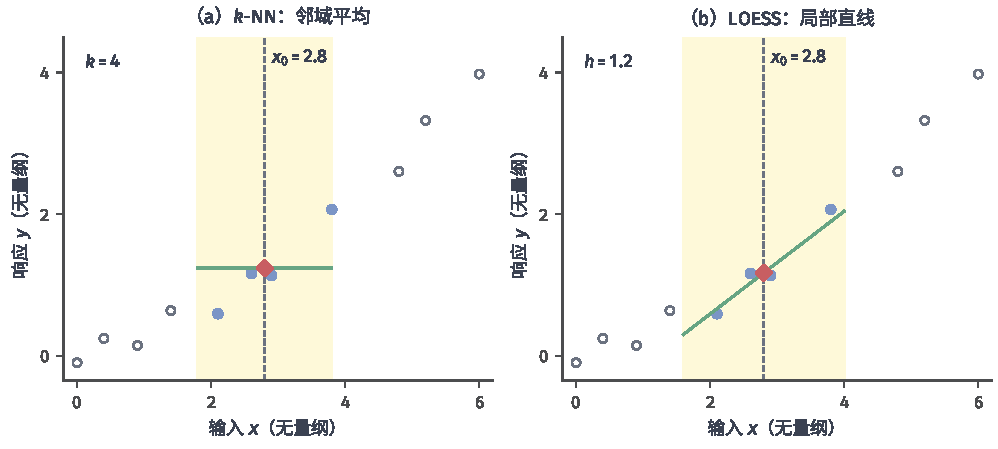
\includegraphics[width=\linewidth]{figures/03-models/01-classic-models/matplotlib/regression-neighborhood/figure.pdf}
  \caption{同一查询点上的邻域平均与局部线性拟合。横、纵轴均无量纲，所有点均为构造样本；空心点为未使用样本，蓝色实心点为本次使用的四个样本，菱形为$x_0=2.8$处的预测。左图取$k=4$、等权平均，预测约为$1.238$；右图取$h=1.2$与三立方距离权重，不做残差重加权，局部线性预测约为$1.171$。浅色带标出各自的邻域，两图同时改变了局部函数形式和权重，不据此断言某种方法总是更准。}
  \label{fig:regression-neighborhood}
\end{figure*}

\subsubsection{参数学习}

设局部基设计为$\bm{P}$，权重矩阵为$\bm{W}=\operatorname{diag}(K_i)$。若$\bm{P}^{\top}\bm{W}\bm{P}$可逆，便可解加权正规方程得到局部系数；实际使用$\bm{W}^{1/2}\bm{P}$的QR分解等方法更合适。邻域无样本或有效点不足以确定多项式时，应扩大邻域、降低阶数或明确回退规则，不能直接使用逆矩阵公式。

一维局部线性形式可写得更清楚。令$u_i=x_i-x_0$，$S_j=\sum_iK_iu_i^j$、$T_j=\sum_iK_iu_i^jy_i$，并记$\Delta=S_0S_2-S_1^2$。方程组为
\[
  \begin{pmatrix}S_0&S_1\\S_1&S_2\end{pmatrix}
  \begin{pmatrix}\widehat a\\\widehat b\end{pmatrix}
  =\begin{pmatrix}T_0\\T_1\end{pmatrix}.
\]
若$\Delta>0$，查询点上的截距可表示为
\begin{equation}
  \widehat m(x_0)=\sum_i l_i y_i,\qquad
  l_i=\frac{K_i(S_2-u_iS_1)}{\Delta}.
  \label{eq:regression-local-linear-weights}
\end{equation}
对非负核权重，$\Delta=\sum_{i<j}K_iK_j(u_i-u_j)^2$，所以至少需要两个不同输入具有正权重。即使$\Delta>0$，接近退化的设计也可能产生很大的$l_i$。

固定带宽与只依赖输入的权重时，估计是响应$\bm{y}$的线性函数。稳健LOESS则在初次拟合后根据残差增加降权系数，再重复局部拟合；权重一旦依赖响应，整体估计便不再是固定的线性平滑算子，下面的固定权重方差公式不能直接沿用。若一个查询使用$n_{\mathrm{loc}}$个有效样本、$q$个局部基函数，稠密拟合约需$O(n_{\mathrm{loc}}q^2+q^3)$运算，另加邻域查询成本。

\subsubsection{理论分析}
\label{sec:regression-loess-theory}

局部线性回归的计算与统计性质都围绕一个固定查询点展开。给定输入后，先考察加权最小二乘是否可解；在一维独立同分布随机设计和确定带宽序列下，再给出依概率的局部偏差方差展开。局部线性再现与渐近展开不能推出无条件风险最优，也不能说明任意稳健重加权实现都会收敛。

\paragraph{收敛性分析}
固定查询点、带宽和邻域权重后，局部多项式拟合是加权最小二乘问题。加权设计满列秩时，求解线性系统即可得到唯一系数；秩亏时则需降阶、正则化或规定回退方式。若加入依赖残差的稳健重加权，外层权重也随拟合改变，单次加权最小二乘的可解性不再等于整个迭代必然收敛，仍需检查相应目标和停止准则。

\paragraph{泛化分析}
局部线性拟合的核心收益是精确再现一次函数。由式\eqref{eq:regression-local-linear-weights}直接求和，
\[
  \sum_i l_i=1,\qquad \sum_i l_i u_i=0.
\]
因此当$m(x)=a+bx$时，$\sum_i l_i m(x_i)=m(x_0)$，不要求样本在$x_0$两侧对称。第二个恒等式解释了局部线性为何能消去一阶趋势造成的偏差。

最终权重$l_i$却不必非负。例如$x_0=0$、$x_1=0.1$、$x_2=0.2$、$K_1=K_2=1$时，$(l_1,l_2)=(2,-1)$。对构造响应$y_i=x_i$，局部线性预测为$0$，局部常数预测为$0.15$。若这两个响应分别加入独立方差为$\sigma^2$的噪声，两种预测的方差则为$5\sigma^2$与$\sigma^2/2$。消除线性偏差需要付出方差代价，不能直接推出局部线性总有更小风险。

更一般地，固定输入且误差条件独立、方差$v(x_i)\leq\sigma^2$时，
\[
  B_n=\sum_i l_i[m(x_i)-m(x_0)],\qquad
  V_n=\sum_i l_i^2v(x_i)
\]
分别为条件偏差和方差。若$m$在覆盖有效邻域的区间二阶连续可微且$|m''|\leq M_2$，用一次项抵消与Taylor余项可得
\[
  |B_n|\leq\frac{M_2}{2}\sum_i|l_i|u_i^2,\qquad
  V_n\leq\sigma^2\sum_i l_i^2.
\]
绝对值不能删去，也不能把这些权重当作凸组合套用$k$-NN回归误差界。

在内部点及规则随机设计下，上述精确公式可进一步化为熟悉的渐近偏差方差展开。局部多项式的系统分析见Fan与Gijbels的专著；下面明确给出本章使用的条件与推导\scite{fan1996local}

以下余项随随机训练输入变化。记$Z_n=o_P(a_n)$表示$Z_n/a_n$依概率趋于零，$Z_n=O_P(a_n)$表示该比值依概率有界：对任意$\delta>0$，存在有限$M$使充分大的$n$满足$\mathbb{P}(|Z_n/a_n|>M)<\delta$。

\Needspace{16\baselineskip}
\begin{theorem}[一维内部点的局部线性展开]
  \label{thm:regression-local-asymptotic}
  设$(X_i,Y_i)$独立同分布，固定内部点$x_0$附近的输入密度$p$连续且$p(x_0)>0$，回归函数$m$二阶连续可微，条件方差$v$在$x_0$连续且有限。核$K$非负、有界、对称，支撑在$[-1,1]$，满足$\int K=1$和$\mu_2=\int u^2K(u)\,du>0$。取确定带宽$h\to0$、$nh\to\infty$，$K_i=K((X_i-x_0)/h)$，记$R(K)=\int K(u)^2du$。在可逆事件上，条件偏差与方差满足
  \begin{align*}
    B_n&=\tfrac12 m''(x_0)\mu_2h^2+o_P(h^2),\\
    V_n&=\frac{v(x_0)R(K)}{nhp(x_0)}+o_P((nh)^{-1}).
  \end{align*}
  可逆事件的概率趋于$1$；在退化事件上须另设估计值。
\end{theorem}

\begin{proof}
令$\mu_j=\int u^jK(u)\,du$。变量替换给出，对$j=0,1,2,3$，
\[
  \frac{\mathbb{E}S_j}{nh^{j+1}}
  =\int u^jK(u)p(x_0+hu)\,du\longrightarrow p(x_0)\mu_j.
\]
局部有界密度与有界紧支撑核给出$\operatorname{Var}(S_j/(nh^{j+1}))=O((nh)^{-1})$，故相应归一化矩依概率趋于$p(x_0)\mu_j$。由$\mu_1=\mu_3=0$，
\[
  \frac{\Delta}{n^2h^4}\xrightarrow{P}p(x_0)^2\mu_2>0,\qquad
  \sum_i l_i u_i^2
    =\frac{S_2^2-S_1S_3}{\Delta}
    =h^2\mu_2+o_P(h^2).
\]
此外$\sum_i|l_i|\leq S_0(S_2+h|S_1|)/\Delta=O_P(1)$。将$m(X_i)$在$x_0$处展开，常数与一次项分别由权重恒等式再现和抵消；二阶连续性使$|u_i|\leq h$内的余项一致为$o(h^2)$，于是得到偏差公式。

为求方差，令$A_j=\sum_iK_i^2v(X_i)u_i^j$，$j=0,1,2$。同样的均值与方差估计给出
\[
  \frac{A_j}{nh^{j+1}}
    \xrightarrow{P}p(x_0)v(x_0)\int u^jK(u)^2du.
\]
把权重公式代入精确条件方差，得到
\[
  V_n=\frac{S_2^2A_0-2S_2S_1A_1+S_1^2A_2}{\Delta^2}.
\]
分子第一项与分母的上述极限给出$v(x_0)R(K)/(nhp(x_0))$，含$S_1$的两项为较小阶，方差公式成立。
\end{proof}

当偏差和方差的领先系数都为正时，平衡$h^4$与$1/(nh)$提示$h$取$n^{-1/5}$量级，对应条件风险的$n^{-4/5}$尺度。若曲率为零，领先偏差项消失，不能仍按同一常数求最佳带宽。这些是随机设计下依概率成立的条件展开；改成无条件均方误差展开还需控制退化设计和余项的可积性。边界点的核矩被截断，也不能直接沿用内部点常数。

\subsubsection{支持局部常数（Nadaraya-Watson 核平滑）}
\label{sec:regression-nadaraya-watson}

在式\eqref{eq:regression-local-polynomial}中只拟合截距，对截距求导便得到\term{Nadaraya--Watson核平滑}（Nadaraya--Watson kernel smoothing）
\begin{equation}
  \widehat m_{\mathrm{NW}}(\bm{x}_0)
  =\frac{\sum_iK_i y_i}{\sum_iK_i},
  \qquad \sum_iK_i>0.
  \label{eq:regression-nw}
\end{equation}
它与局部多项式使用相同的邻域权重，但只作加权平均。Nadaraya与Watson分别研究了这一核回归路线；具体带宽和设计条件仍须与所用理论结果对应\scite{nadaraya1964,watson1964}

在联合密度存在的设定下，$m(x)p(x)=\int y\,p(x,y)\,dy$，所以归一化核响应和可估计$m(x)p(x)$，核计数可估计$p(x)$，比值便近似条件均值。

局部常数权重和为$1$，但通常不满足一阶矩为零。因此一侧邻域的斜率可能带来一阶偏差。以一维内部点为例，把经验核和换为总体积分，记总体平滑值为$m_h(x_0)$。在$m,p$二阶连续可微、$p(x_0)>0$及前述对称紧支撑核条件下，对分子$\int K(u)m(x_0+hu)p(x_0+hu)\,du$和分母$\int K(u)p(x_0+hu)\,du$分别展开，得到
\[
  m_h(x_0)-m(x_0)
  =\mu_2h^2\left[\frac{m''(x_0)}{2}
       +\frac{m'(x_0)p'(x_0)}{p(x_0)}\right]+o(h^2).
\]
后一项反映设计密度不均匀的影响。局部线性消去这项并改善边界处的一阶偏差，但其负权重可能增大方差，所以选择仍应看总风险。

\subsubsection{小结}

LOESS用局部斜率或曲率补充局部平均，适合观察低维输入与响应之间的平滑关系。其有效性取决于局部数据量、设计秩、带宽和光滑程度；稳健重加权可以减轻部分异常响应影响，却没有消除所有异常点风险。它不提供一组统一的全局斜率，但局部曲线和局部导数仍有解释价值，不能简单等同于“不可解释”。

\subsection{模型对比与总结}

$k$-NN回归与LOESS都根据查询点选择局部数据，差别在于是否拟合邻域内的趋势。$k$-NN回归的均匀权重便于控制方差，局部线性权重能再现一次函数，却可能为负。内部点、边界点、对称设计与不均匀设计下，两者的偏差阶并不总相同，因此不能无条件声称LOESS的风险严格小于$k$-NN回归。

平滑样条沿另一条路线控制函数曲率，径向基函数网络则先选中心再学习全局展开系数。它们与邻域方法都使用局部性或相似性，但目标并不相同。尤其Nadaraya--Watson的系数由查询点归一化得到，核岭回归的训练系数则由整个Gram矩阵耦合求解；二者一般不等价。选择方法时应同时考虑局部光滑性、输入的有效维数和查询预算，而不是把所有带核权重的方法视为同一个模型。

\section{基于树与规则的回归}
\label{sec:regression-trees}

第\ref{sec:classic-overview-tree-rules}节已经给出条件分支与区域预测的共同结构。本节关注回归时怎样按响应损失选择区域，并确定叶内预测。CART采用递归划分，模型树在叶内加入线性趋势，MARS用连续铰链基表达阈值及交互。MARS的基函数可以重叠，并不构成标准决策树；把它放在这里，是为了比较不同的条件与分段表达。

\subsection{CART 回归树}
\label{sec:regression-cart}

\term{分类与回归树}（classification and regression trees, CART）将递归二分、叶内估计和复杂度剪枝组织成统一框架。Breiman等人在1984年的专著中系统阐述了这套方法，把数据决定的分区与树的规模控制联系起来。回归情形通常用平方误差评价分裂，再通过独立验证选择树的规模；这一流程将在下面分别展开\scite{breiman1984cart}

第\ref{sec:classification-cart}节的分类CART共享递归二分与代价复杂度剪枝。任务差异落在分裂和叶输出上：本节按响应平方误差选择分区并输出叶均值，分类树按类别不纯度或误分类代价分裂，并输出类别标签或类别比例。

\subsubsection{模型结构}

设树$T$的叶区域为$R_1,\ldots,R_M$，则
\begin{equation}
  f_T(\bm{x})=\sum_{m=1}^{M}c_m\mathbf{1}\{\bm{x}\in R_m\}.
  \label{eq:regression-cart-model}
\end{equation}
数值特征上的节点规则通常为$x_j\leq s$与$x_j>s$，递归后形成轴对齐区域；类别特征则可按类别子集分支，不宜继续称为普通欧氏矩形。缺失值并非由树结构自动解决，还需指定缺失方向或其他规则。例如，\term{替代分裂}（surrogate split）在主测试特征缺失时，用其他特征的测试尽量复现主分裂的左右分配。

固定非空叶的样本索引集$I_m$后，令$\bar y_m=|I_m|^{-1}\sum_{i\in I_m}y_i$，有
\[
  \sum_{i\in I_m}(y_i-c)^2
  =\sum_{i\in I_m}(y_i-\bar y_m)^2+|I_m|(c-\bar y_m)^2.
\]
因此$c_m=\bar y_m$在平方损失下最优。改用绝对或分位数损失时，叶预测相应变为中位数或分位数；模型结构与损失选择仍然可以分开。

图\ref{fig:regression-tree-prediction}把一棵给定的阈值树展开为预测函数。沿树走到同一叶的输入共享一个预测值，所以一维常数叶回归树产生水平分段，而阈值处可以跳跃。图中每个叶的数值都来自该叶的两条响应，后面的学习问题才是如何从候选阈值中选出这些分区。

\begin{figure*}[t]
  \centering
  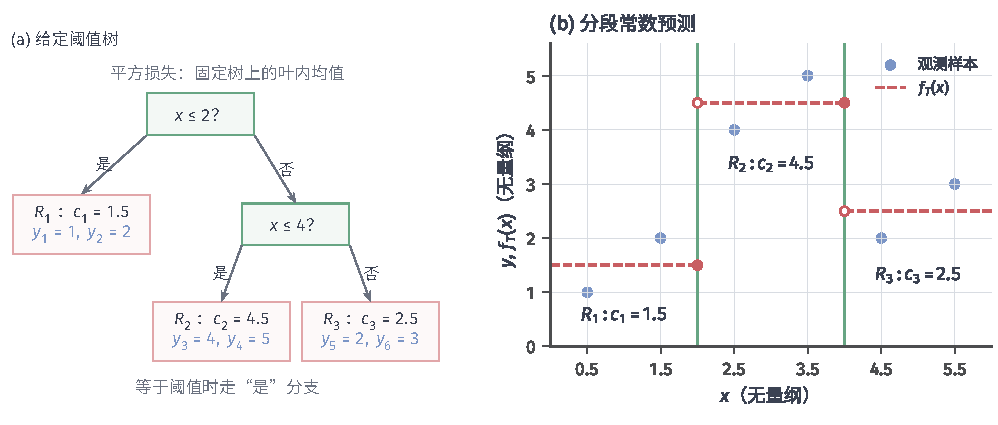
\includegraphics[width=\linewidth]{figures/03-models/01-classic-models/matplotlib/regression-tree-prediction/figure.pdf}
  \caption{给定阈值树与分段常数预测。六个无量纲教学样本按$x$递增排列；按$x\leq2$及右分支上的$x\leq4$划分后，三组响应分别为$(1,2)$、$(4,5)$、$(2,3)$，叶均值为$1.5$、$4.5$、$2.5$。蓝色点表示样本，红色虚线表示预测，绿色竖线表示阈值；阈值处实心、空心端点区分取与不取该值。右图只显示$0\leq x\leq6$，树结构预先给定。}
  \label{fig:regression-tree-prediction}
\end{figure*}

\subsubsection{参数学习}
\label{sec:regression-cart-learning}

在当前节点内，算法枚举特征与候选阈值，选择子节点平方误差和最小的分裂。对两个非空子节点，记样本数为$n_L,n_R$，均值为$\bar y_L,\bar y_R$，则分裂增益可精确写成
\begin{equation}
  \Delta_{\mathrm{split}}
  =\mathrm{SSE}_{\mathrm{parent}}
    -\mathrm{SSE}_{L}-\mathrm{SSE}_{R}
  =\frac{n_Ln_R}{n_L+n_R}(\bar y_L-\bar y_R)^2.
  \label{eq:regression-cart-gain}
\end{equation}
证明只需把两个子节点响应分别围绕自己的均值展开，再利用父均值为加权平均。该式说明增益同时考虑两组均值差异和样本量。

连续特征只需在相邻不同取值之间设候选切分，排好序后用累计和、平方和更新各侧SSE。类别子集有更多候选；在无额外分裂约束的平方误差二分问题中，可先按类别响应均值排序再考虑相邻分组，但带最小样本数、权重或其他限制时须重新检查相应结论。停止条件可限制最大深度、最小叶样本数和最低增益。贪心选择只保证当前节点在候选集中的最佳切分，不保证整棵树全局最优。

树生长后，用叶数惩罚控制规模。固定一个已生长的有限二叉树$T_0$，对其剪枝子树$T$定义
\begin{equation}
  R_\alpha(T)=\sum_{m\in\operatorname{leaves}(T)}
                    \mathrm{SSE}_m+\alpha|\operatorname{leaves}(T)|,
  \qquad\alpha\geq0.
  \label{eq:regression-pruning}
\end{equation}
\term{代价复杂度剪枝}（cost-complexity pruning）在保留局部拟合与减少叶数之间作折中。临界$\alpha$处可能出现多个最优子树，唯一性需要额外的并列规则。

\Needspace{11\baselineskip}
\begin{theorem}[固定生长树内的最优剪枝]
  \label{thm:regression-pruning}
  设$Q_\alpha(v)$为从$T_0$的节点$v$出发可得到的所有剪枝子树的最小代价。若$v$是原始叶，则$Q_\alpha(v)=\mathrm{SSE}_v+\alpha$；若$v$有左右孩子$v_L,v_R$，则
  \[
    Q_\alpha(v)=\min\{\mathrm{SSE}_v+\alpha,\,
                     Q_\alpha(v_L)+Q_\alpha(v_R)\}.
  \]
  从叶到根计算该递推，并保存每次选择，可得到$R_\alpha$的最优剪枝子树。
\end{theorem}

\begin{proof}
原始叶无其他选择，结论成立。对内部节点，任何合法剪枝子树要么把$v$收缩为一片叶，要么保留分裂。前者代价为$\mathrm{SSE}_v+\alpha$；后者的两个孩子可以独立剪枝，代价相加，归纳假设给出最小和为$Q_\alpha(v_L)+Q_\alpha(v_R)$。这两类穷尽全部选择，因此取最小值即可。相等时两个选择都最优，记录任一个并列规则均可返回一个最优解。
\end{proof}

固定$\alpha$时，递推只需对每个节点作常数次比较，因此在节点SSE已知后为$O(|T_0|)$。经典最弱环节方法进一步构造随$\alpha$变化的嵌套剪枝路径，再通过验证选择规模；它优化的仍是给定生长树内的剪枝集合，而不是所有可能的树。交叉验证时，各折的生长与剪枝都应仅使用该折训练集。

\subsubsection{理论分析}
\label{sec:regression-cart-theory}

树模型需要分开回答“有限训练集上的建树与剪枝何时结束”和“叶内预测怎样推广到新样本”。前一个问题给出有限步计算结论；后一个问题在结构样本与估计样本独立时，考察固定查询点的条件期望误差及附加条件下的一致性。两类结果都不能推出普通响应自适应CART在任意数据分布上的泛化保证。

\paragraph{收敛性分析}
在有限训练集上，若每次分裂都产生两个非空子节点，叶数至多为$n$，树的生长会在有限步内终止。对固定生长树，前述剪枝递推也能在有限步内求得该树内的最优剪枝。这些计算性质没有把逐节点贪心搜索变成所有树结构上的全局优化，也没有回答样本量增加时的预测误差是否趋于零。

\paragraph{泛化分析}
固定分区后的叶均值看起来类似$k$-NN回归的局部平均，但普通CART使用同一批响应选择分裂并估计均值。条件于最终分区，不会自动使被选中的噪声重新保持零均值。分析响应自适应分区需要控制分区类和选择过程，Nobel关于数据依赖分区的工作正是从这类条件出发；仅写“叶直径趋零、样本数趋无穷”不能代替完整定理\scite{nobel1996partitions}

用独立数据分别选分区和估计叶均值，可以得到一个透明的有限样本结论。\term{诚实分区}（honest partitioning）在这里指：结构样本决定分区，独立估计样本提供叶内被平均的响应。

\Needspace{14\baselineskip}
\begin{theorem}[独立分区下的叶平均误差]
  \label{thm:regression-honest-tree}
  用结构样本选定可测分区$\Pi$，用独立同分布的估计样本计算叶均值。假设估计样本满足零条件均值噪声、条件方差不超过$\sigma^2$，回归函数$m$为$L$-Lipschitz。固定查询点$\bm{x}$，其叶为$A$，其中估计样本数为$N_A$，叶内最大样本距离为$R_A$。条件于结构样本与全部估计输入的信息$\mathcal G$，在$N_A>0$时，
  \[
    \mathbb{E}[(\widehat m_\Pi(\bm{x})-m(\bm{x}))^2\mid\mathcal G]
    \leq L^2R_A^2+\frac{\sigma^2}{N_A}.
  \]
  若空叶预测规定为零，则$N_A=0$时的条件误差为$m(\bm{x})^2$。
\end{theorem}

\begin{proof}
条件于$\mathcal G$，分区与叶成员已固定，估计响应的噪声仍条件独立且均值为零。非空叶内误差拆为$m$值之差的平均与噪声平均；前者绝对值不超过$LR_A$，后者方差不超过$\sigma^2/N_A$，交叉项期望为零。空叶使用预定值零，误差直接为$m(\bm{x})^2$。
\end{proof}

在有界$m$下，若$R_A\to0$、$N_A\to\infty$依概率成立，可用与$k$-NN回归相同的有界偏差分解和噪声界得到点态均方一致性。空叶概率随之趋零。这里的样本数是独立估计样本中的叶成员数，结构样本上的最小叶样本约束并不自动保证它。

普通CART不能直接套用这一界。考虑固定输入$(1,2,3)$、查询点$2$，真实$m\equiv0$，三个响应独立等概率取$\pm1$。令树必须在$1.5$和$2.5$之间择一分裂，查询叶始终含两个样本。只要左邻或右邻与中间响应同号，最小SSE切分就选到同号二点叶，预测平方为$1$；该事件概率为$3/4$。两侧均异号时预测为零，故实际风险为$3/4$，大于机械套用$\sigma^2/N_A$得到的$1/2$。该反例否定的是独立平均公式的直接挪用，并不声称所有CART程序都不一致。

有限样本下，单棵树还可能对数据扰动敏感，贪心分裂也可能错过只有联合出现才有效的交互。后续的Bagging、随机森林和梯度提升通过多棵树组合改善某些误差来源，但具体改善仍依赖数据与训练设定，不能把集成当作无条件消除偏差或方差的步骤。

\subsubsection{支持分段线性叶节点（模型树 M5）}
\label{sec:regression-model-tree}

如果每个区域内的价格趋势近似线性，用多片常数叶逼近可能需要很多切分。\term{模型树}（model tree）在叶内拟合线性模型$f_m(\bm{x})=b_m+\bm{w}_m^{\top}\bm{x}_{A_m}$，其中$A_m$为该叶使用的特征集。M5是这条路线的代表，用树选择适用区域，再用局部回归描述区域内部的趋势\scite{quinlan1992m5}

局部样本少时，叶内设计可能秩亏，需要选择变量或正则化。父子节点预测的加权混合可以缓和估计跳跃，但两侧叶模型在共同边界上没有被强制相等，因此这种平滑处理不自动保证函数连续。叶模型也可改为GLM、岭或Lasso，不过分裂准则、参数估计与复杂度惩罚需要与新模型配套，不能只替换叶公式就沿用全部CART理论。

\subsubsection{小结}

CART把回归拆为选分区与叶内估计，阈值规则适合表达局部条件关系。它对输入单位缩放通常不如距离方法敏感，但候选分裂数量、缺失值规则与叶内样本量仍会影响结果。固定生长树内的剪枝可以精确优化，整体建树仍是贪心搜索；同一响应参与选树的自适应性也必须进入统计分析。

\subsection{多元自适应回归样条（MARS）}
\label{sec:regression-mars}

树的阈值选择能够适应数据，常数叶却在边界处跳跃。\term{多元自适应回归样条}（multivariate adaptive regression splines, MARS）把阈值写进连续的铰链基函数，再从数据中选择这些基函数及其乘积。Friedman在1991年提出这一方法，将自适应选择结点与样条展开结合。它在可加模型与树式区域表达之间提供了另一种选择：多个基函数可同时作用于同一输入，预测不再由唯一一片叶决定\scite{friedman1991mars}

\subsubsection{模型结构}

对特征$x_j$与结点$t$，\term{铰链函数}（hinge function）为$(x_j-t)_+$与$(t-x_j)_+$，它们在结点一侧为零，另一侧线性变化。MARS写成
\begin{equation}
  f(\bm{x})=\beta_0+\sum_{m=1}^{M}\beta_m B_m(\bm{x}),
  \qquad
  B_m(\bm{x})=\prod_{l=1}^{q_m}
                 [s_{m,l}(x_{j_{m,l}}-t_{m,l})]_+,
  \label{eq:regression-mars}
\end{equation}
其中$s_{m,l}\in\{-1,1\}$，$q_m$为该基的因子数。通常限制最高交互阶数，并对同一乘积中重复使用变量设规则，避免无约束扩张。

单个铰链连续但在结点不可微；含两个不同变量的乘积如$(x_1-3)_+(5-x_2)_+$在激活区域是二次乘积，不再是整体分段线性函数。铰链和乘积都连续，所以有限线性组合连续，但可微性需要额外平滑构造。严格加性版本只允许单变量基，增加乘积则允许指定阶数内的交互。

\subsubsection{参数学习}

前向阶段从常数模型开始，在当前基函数$B_l$、候选变量$j$与候选结点$t$中搜索，将$B_l(\bm{x})(x_j-t)_+$和$B_l(\bm{x})(t-x_j)_+$成对加入，并重新拟合线性系数。选择使训练平方误差下降最多的候选，直到达到基数、交互阶数或改善量限制。结点与基函数都由响应参与选择，因此整个训练过程不同于固定设计的一次OLS。

后向阶段逐个尝试删除非截距基函数，每次保留训练误差增加最小的删除，构造不同规模的模型序列。再从序列中按验证误差或广义交叉验证选模型，而不是一看到GCV不再下降就必然停止搜索。常用准则写成
\begin{equation}
  \operatorname{GCV}
  =\frac{\mathrm{SSE}/n}{(1-C_{\mathrm{eff}}/n)^2},
  \qquad C_{\mathrm{eff}}<n.
  \label{eq:regression-mars-gcv}
\end{equation}
$C_{\mathrm{eff}}$是复杂度计数，既考虑保留的线性系数，也以附加惩罚近似结点搜索的代价。例如可写成$q+cK$，其中$q$是保留设计的秩，$K$是采用相应计数约定的结点数，$c$是每个结点的附加代价。软件对成对基、交互结点与自由度有不同计数方式，不能把它一律写成“输入维数乘基数”，更不能视为数据自适应拟合的精确自由度。

\subsubsection{理论分析}

MARS先在固定候选集合中作前向与后向搜索，随后才面对响应参与基选择所产生的统计误差。有限搜索只能给出算法终止和局部改进；要控制后者，还需对独立同分布样本、函数空间增长与模型选择另加条件。因此，有限步停止不能推出全局最优，样条空间的理论也不能直接推出默认MARS贪心程序的风险界。

\paragraph{收敛性分析}
固定基函数后，系数可通过最小二乘求解。前向搜索在给定基数量上限或满足停止准则时结束，后向阶段每步删除基函数，也会在有限步内终止。前向与后向步骤都没有搜索全部可能基集合，因此不能由每一步的局部改善推出全局最优。

\paragraph{泛化分析}
如果基函数由同一批响应选择，直接条件于所选设计再套用固定设计OLS的无偏性，就忽略了选择偏差。统计分析需要同时考虑系数估计与基函数选择。

样条与低阶交互函数空间有成熟的逼近和统计理论。例如，扩展线性建模研究了多项式样条及张量积表示怎样适应指定的低阶结构。但这类结果中的空间增长、平滑性和模型选择条件必须逐项核对，不能直接变成某个默认MARS贪心实现的极小极大保证\scite{stone1997splines}

MARS输出连续函数并不意味着其估计方差必小于CART。结点选择可以对样本扰动敏感，多个铰链也可能高度相关。实践中可限制交互阶数和基数量，并用独立验证比较预测；对数据范围外的外推尤其应检查，铰链的线性增长可能在缺少观测支持处产生较大的预测值。

\subsubsection{小结}

MARS通过自适应结点与铰链乘积表达阈值和交互，在线性系数层面仍可使用最小二乘。其连续性来自基函数，灵活性来自基选择；这两者分别对应表示与搜索问题。限制交互能减少候选复杂度，也可能遗漏真实关系，是否合适应由任务和数据判断。

\subsection{模型对比与总结}

CART用不重叠叶区域和常数预测，模型树在叶内增加线性趋势，MARS用可重叠的连续基函数及其乘积。前两者沿树路径路由，MARS需要计算保留的基；叶线性模型可能在边界跳跃，MARS的基本铰链构造则连续但不必处处可微。三者都允许阈值由数据决定，却使用不同的复杂度控制。

相关工作还从选择偏差和集成方式改进树模型。\term{条件推断树}（conditional inference tree）把变量关联检验与分裂位置选择分开，缓解候选切分多的变量更容易被选中的偏向；检验规则和显著性水平仍会影响树大小，不能理解为自动杜绝过拟合\scite{hothorn2006ctree}

\section{基于概率的回归}
\label{sec:regression-probabilistic}

本节接续第\ref{sec:classic-overview-probabilistic}节的概率视角，具体计算未知系数或函数的后验，以及未来响应的预测分布。GLM已经为响应指定条件分布；这里重点保留参数或函数估计的不确定性，并与响应噪声区分。

\term{分布回归}（distributional regression）提供了完整条件分布的另一条入口：先选择响应分布族，再让位置、尺度或形状等多个分布参数分别依赖输入。GAMLSS允许用线性项或平滑项建模这些参数，因而能表达均值不变但条件方差、偏度或尾部随输入变化的情形\scite{rigby2005gamlss}它与只拟合若干分位点不同，也不等同于描述未知函数后验的GPR；代价是必须选择分布族、链接与各参数的结构，并用适当评分和校准诊断检查整个预测分布。

\subsection{高斯过程回归（GPR）}
\label{sec:regression-gpr}

\term{高斯过程回归}（Gaussian process regression, GPR）通过均值函数和协方差函数规定未知函数在任意有限输入集合上的联合分布。高斯观测噪声使后验与预测分布可以精确计算；权重空间与函数空间两种推导也把它与贝叶斯线性回归、核岭回归联系起来。

高斯过程预测较早已用于时间序列和地统计学，空间预测中的相关方法通常称为克里金（kriging）。20世纪90年代，Williams与Rasmussen在机器学习语境中讨论了GPR及协方差函数参数的学习，并将它与贝叶斯神经网络联系起来\scite{rasmussen2006}

\subsubsection{模型结构}
\label{sec:regression-gpr-structure}

先考虑有限维特征$\bm{\phi}(\bm{x})\in\mathbb{R}^{p}$，令$f(\bm{x})=\bm{\phi}(\bm{x})^{\top}\bm{w}$。与OLS把$\bm{w}$看作待估计固定量不同，\term{贝叶斯线性回归}（Bayesian linear regression）对$\bm{w}$设置分布，再根据数据更新。使用高斯先验与高斯噪声，更新可通过完成平方得到。

\Needspace{14\baselineskip}
\begin{theorem}[贝叶斯线性回归的后验与预测]
  \label{thm:regression-bayesian-linear}
  条件于设计矩阵$\bm{X}$，设$\bm{w}\sim\mathcal{N}(\bm{m}_0,\bm{V}_0)$，其中$\bm{V}_0\succ0$，并设$\bm{y}=\bm{X}\bm{w}+\bm{\varepsilon}$，$\bm{\varepsilon}\sim\mathcal{N}(\bm{0},\sigma^2\bm{I})$与$\bm{w}$独立，$\sigma^2>0$。则
  \[
    \begin{aligned}
      \bm{V}_n&=(\bm{V}_0^{-1}+\sigma^{-2}\bm{X}^{\top}\bm{X})^{-1},\\
      \bm{m}_n&=\bm{V}_n
          (\bm{V}_0^{-1}\bm{m}_0+\sigma^{-2}\bm{X}^{\top}\bm{y}),
    \end{aligned}
  \]
  且$\bm{w}\mid\bm{X},\bm{y}\sim\mathcal{N}(\bm{m}_n,\bm{V}_n)$。新响应采用独立同方差噪声时，
  \[
    Y_{\star}\mid\bm{x}_{\star},\bm{X},\bm{y}
    \sim\mathcal{N}\bigl(
      \bm{\phi}_{\star}^{\top}\bm{m}_n,\,
      \bm{\phi}_{\star}^{\top}\bm{V}_n\bm{\phi}_{\star}+\sigma^2\bigr).
  \]
\end{theorem}

\begin{proof}
先验与似然的负对数相加，去掉与$\bm{w}$无关的项后为
\[
  \tfrac12\bm{w}^{\top}
       (\bm{V}_0^{-1}+\sigma^{-2}\bm{X}^{\top}\bm{X})\bm{w}
  -\bm{w}^{\top}
       (\bm{V}_0^{-1}\bm{m}_0+\sigma^{-2}\bm{X}^{\top}\bm{y}).
\]
定义定理中的$\bm{V}_n,\bm{m}_n$，上式等于
$\tfrac12(\bm{w}-\bm{m}_n)^{\top}\bm{V}_n^{-1}(\bm{w}-\bm{m}_n)$加常数。精度矩阵正定，故该可积密度归一化后就是所述高斯后验。新响应为后验高斯参数的线性变换与独立高斯噪声之和，均值与方差相加即得预测分布。
\end{proof}

若只需用一个参数向量概括后验，沿用
\BookSectionRef{sec:statistics-bayes-hierarchy}{第一卷“数学准备”的“有限维目标的估计”小节}
中的最大后验估计（MAP）。固定设计与超参数，且最大值能够取到时，当前回归模型的目标为
\begin{equation}
  \begin{aligned}
    \widehat{\bm{w}}_{\mathrm{MAP}}
      &\in\argmax_{\bm{w}}p(\bm{w}\mid\bm{X},\bm{y})\\
      &=\argmax_{\bm{w}}
        \{\log p(\bm{y}\mid\bm{X},\bm{w})+\log p(\bm{w})\}.
  \end{aligned}
  \label{eq:regression-map}
\end{equation}
后验的归一化常数与$\bm{w}$无关，因而不影响最大化。MAP使用后验众数，后验均值则对参数按后验加权平均，两者一般不同。

图~\ref{fig:regression-mle-map-geometry}在二维参数平面上展示这两个目标的差别。似然单独把最优点放在数据偏好的中心；零均值先验则偏好靠近原点的参数。MAP最小化负对数似然与负对数先验之和，因此落在二者共同决定的位置，而不是在MLE与先验中心之间任意作线性插值。椭圆形状和先验尺度改变时，折中的方向也会改变。
\begin{figure}[htbp]
  \centering
  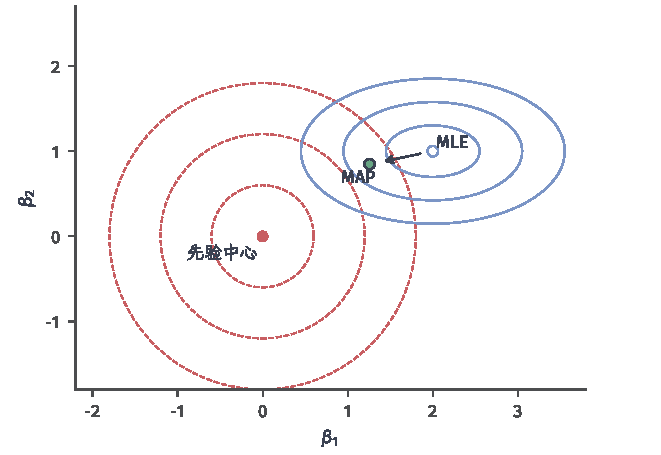
\includegraphics[width=\linewidth]{figures/03-models/01-classic-models/matplotlib/regression-mle-map-geometry/figure.pdf}
  \caption{MLE与MAP的参数几何。蓝色实线是以$(2,1)^\top$为中心、两坐标尺度分别为$1$和$0.55$的高斯似然等高线；红色虚线是以原点为中心、尺度为$1.3$的各向同性高斯先验等高线。空心点为MLE，绿色实心点为两项相加后的MAP $(1.256,0.848)^\top$。该构造用于显示先验如何改变点估计，不代表MAP总在两中心的连线上。}
  \label{fig:regression-mle-map-geometry}
\end{figure}

若$\bm{m}_0=\bm{0}$、$\bm{V}_0=\tau^2\bm{I}$，后验均值为$(\bm{X}^{\top}\bm{X}+\sigma^2\bm{I}/\tau^2)^{-1}\bm{X}^{\top}\bm{y}$，在本章归一化下对应$\lambda=\sigma^2/(n\tau^2)$的岭估计。高斯后验的均值与众数相同，所以也等于MAP估计。该对应要求截距处理一致：若先验惩罚全部特征系数，就不能直接与截距不受惩罚的岭模型比较。后验协方差与前面固定真参数下岭估计的重复抽样协方差也是不同对象。

有限维贝叶斯线性模型已经诱导出函数上的高斯分布：
\[
  m_0(\bm{x})=\bm{\phi}(\bm{x})^{\top}\bm{m}_0,\qquad
  k(\bm{x},\bm{x}')=\bm{\phi}(\bm{x})^{\top}\bm{V}_0\bm{\phi}(\bm{x}').
\]
任意有限个函数值都是高斯参数的线性变换，因此联合高斯。直接指定$m_0$和正定核$k$，便可越过显式系数建立函数先验。

沿用\BookSectionRef{sec:rv-finite-dimensional-laws}{第一卷“数学准备”的随机过程有限维联合分布小节}
与\BookSectionRef{sec:rv-paths}{第一卷“数学准备”的高斯过程小节}，
把这些相容的高斯分布记为$f\sim\mathcal{GP}(m_0,k)$：任意有限输入集合上的函数值向量联合高斯。
正定核保证有限协方差矩阵半正定，扩张定理据此建立过程；
是否具有连续样本路径还需额外条件，不能由核的正定性直接推出。

高斯过程允许有限秩核，因此并不必然对应无限维特征；有限维贝叶斯线性回归正是其中一个特例。对无限维核，也不需要先假设存在协方差为无限维单位矩阵的普通高斯权重向量，定义有限函数值的相容联合分布即可。

加入与函数独立的噪声$y_i=f(\bm{x}_i)+\varepsilon_i$，其中$\varepsilon_i$相互独立且服从$\mathcal{N}(0,\sigma^2)$，$\sigma^2>0$。令$\bm{K}_{i,j}=k(\bm{x}_i,\bm{x}_j)$，$(\bm{k}_{\star})_i=k(\bm{x}_i,\bm{x}_{\star})$，$\bm{m}_0$表示训练点上的先验均值向量，$\bm{C}=\bm{K}+\sigma^2\bm{I}$，$f_{\star}=f(\bm{x}_{\star})$。联合分布为
\[
  \begin{pmatrix}\bm{y}\\f_{\star}\end{pmatrix}
  \sim\mathcal{N}\!\left[
    \begin{pmatrix}\bm{m}_0\\m_0(\bm{x}_{\star})\end{pmatrix},
    \begin{pmatrix}
      \bm{C}&\bm{k}_{\star}\\
      \bm{k}_{\star}^{\top}&k(\bm{x}_{\star},\bm{x}_{\star})
    \end{pmatrix}\right].
\]
于是后验预测可以精确写成
\begin{equation}
  \begin{aligned}
    \mu_{\star}
      &=m_0(\bm{x}_{\star})
        +\bm{k}_{\star}^{\top}\bm{C}^{-1}(\bm{y}-\bm{m}_0),\\
    v_{\star}
      &=k(\bm{x}_{\star},\bm{x}_{\star})
        -\bm{k}_{\star}^{\top}\bm{C}^{-1}\bm{k}_{\star}.
  \end{aligned}
  \label{eq:regression-gp-posterior}
\end{equation}
为证明它，令$Z=f_{\star}-m_0(\bm{x}_{\star})-\bm{k}_{\star}^{\top}\bm{C}^{-1}(\bm{y}-\bm{m}_0)$。直接计算得到$\operatorname{Cov}(Z,\bm{y})=\bm{0}$；$Z$与$\bm{y}$联合高斯，所以独立。其方差为$v_{\star}$，从而条件于$\bm{y}$时，$f_{\star}$的均值为$\mu_{\star}$、方差为$v_{\star}$。该方差非负也由它是随机变量方差得到。未来带噪声响应的方差则为$v_{\star}+\sigma^2$。

核选择规定了先验中的相似性。平方指数核$k(\bm{x},\bm{x}')=\sigma_f^2\exp(-\lVert\bm{x}-\bm{x}'\rVert_2^2/(2\ell^2))$具有很强的平滑性，其中$\sigma_f^2>0$是信号方差、$\ell>0$是长度尺度。Matérn核可调节平滑程度，例如$\nu=3/2$时为$\sigma_f^2(1+\sqrt3r/\ell)\exp(-\sqrt3r/\ell)$，其中$r=\lVert\bm{x}-\bm{x}'\rVert_2$，对应一次均方可微的过程。一维周期核可写成$\sigma_f^2\exp(-2\sin^2(\pi(x-x')/p)/\ell^2)$，表达周期$p>0$的相关结构。合法核的和与乘积仍合法，可以组合趋势与周期，但不保证所组合的结构符合实际数据。

图\ref{fig:regression-gp-posterior}展示了式\eqref{eq:regression-gp-posterior}的两项输出。在这个固定平稳核的例子中，观测附近的函数值受到较强约束，观测间的较大空隙与远离观测的区域保留更多不确定性。曲线给出点预测，带状区域则说明在当前先验和噪声设定下，哪些函数值仍与数据相容。

\begin{figure}[htbp]
  \centering
  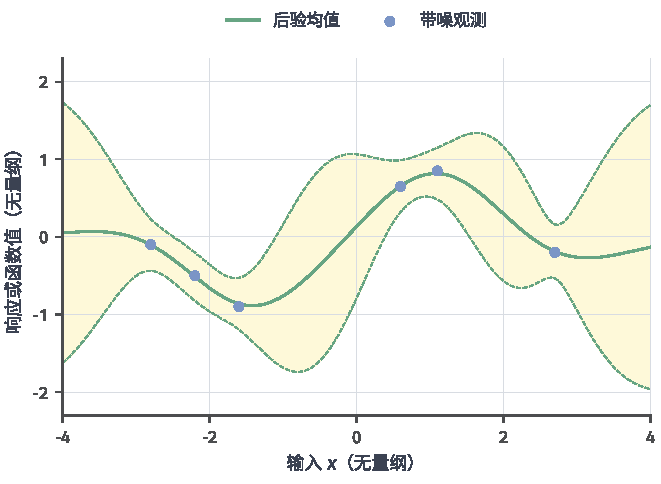
\includegraphics[width=\linewidth]{figures/03-models/01-classic-models/matplotlib/regression-gp-posterior/figure.pdf}
  \caption{高斯过程的后验均值与函数不确定性。六个点为构造观测；先验均值为零，平方指数核取$\ell=0.9$、$\sigma_f=1$，观测噪声标准差为$\sigma=0.18$。实线为$\mu_{\star}$，浅色带及虚线边界为$\mu_{\star}\pm1.96\sqrt{v_{\star}}$，表示潜在函数值的逐点约$95\%$后验可信区间。它不是整条函数的同时可信带；预测未来带噪响应时，方差还须加$\sigma^2$。}
  \label{fig:regression-gp-posterior}
\end{figure}

\subsubsection{参数学习}
\label{sec:regression-gpr-learning}

给定核和噪声参数时，后验已经由式\eqref{eq:regression-gp-posterior}确定；仍需选择长度尺度、信号方差、噪声方差及可能的均值参数。令这些超参数为$\bm{\theta}$，把训练输入处的潜在函数值积分掉，得到\term{边缘似然}（marginal likelihood）：在给定输入和超参数时，观测响应向量的概率密度。以下令先验均值为零：
\begin{equation}
  \log p(\bm{y}\mid\bm{X},\bm{\theta})
   =-\tfrac12\bm{y}^{\top}\bm{C}_{\bm{\theta}}^{-1}\bm{y}
    -\tfrac12\log|\bm{C}_{\bm{\theta}}|
    -\tfrac n2\log(2\pi).
  \label{eq:regression-gp-evidence}
\end{equation}
二次项评价响应与协方差结构的匹配，行列式项来自密度归一化，两者共同决定目标。不能把“更复杂的核”机械等同于“行列式更大”，也不能由边缘似然推出自动找到正确结构或无需验证。

若$\bm{a}=\bm{C}^{-1}\bm{y}$，固定零均值模型的梯度为
\[
  \frac{\partial\log p(\bm{y})}{\partial\theta_j}
  =\tfrac12\operatorname{tr}\!\left[
    (\bm{a}\bm{a}^{\top}-\bm{C}^{-1})
    \frac{\partial\bm{C}}{\partial\theta_j}\right].
\]
它来自$d\bm{C}^{-1}=-\bm{C}^{-1}(d\bm{C})\bm{C}^{-1}$与$d\log|\bm{C}|=\operatorname{tr}(\bm{C}^{-1}d\bm{C})$。可以在正参数的对数坐标上使用梯度算法，多初值比较有助于发现不同局部最优；这种经验贝叶斯拟合通常仍把所选超参数当作固定值，因此没有保留全部超参数不确定性。

数值计算使用Cholesky分解$\bm{C}=\bm{L}\bm{L}^{\top}$。解两次三角方程得到$\bm{a}$后，预测均值为$\bm{k}_{\star}^{\top}\bm{a}$；令$\bm{v}=\bm{L}^{-1}\bm{k}_{\star}$，预测方差为$k(\bm{x}_{\star},\bm{x}_{\star})-\lVert\bm{v}\rVert_2^2$。稠密分解需要$O(n^3)$时间、$O(n^2)$存储，预计算后的单点均值需$O(n)$算术加核计算，单点方差通常需$O(n^2)$三角求解。均值与方差不能统称同一个预测代价。

大数据下可选取$m\ll n$个输入位置$\bm{z}_j$，以潜在函数值$u_j=f(\bm{z}_j)$作为\term{诱导变量}（inducing variables），通过它们的近似后验概括数据对函数的约束。Titsias的变分诱导点方法在高斯回归中优化边缘对数似然的变分下界，以选择诱导输入并近似后验，常见稠密计算规模为$O(nm^2)$；后续随机变分方法进一步支持小批量训练。近似是否充分，仍需检查诱导表示能否保留任务所需的函数变化\scite{titsias2009}

\subsubsection{理论分析}
\label{sec:regression-gpr-theory}

GPR内部的线性系统求解与样本增加时的后验收缩是两个层次的问题。固定设计、固定核和正噪声方差给出后验线性系统与正则化函数解的确定性最优性；明确回归抽样制度、真函数光滑性和先验尺度后，才可讨论渐近后验集中。这些结论不能推出经验贝叶斯超参数选择后的频率覆盖，也不能保证模型失配时的预测区间有效。

\paragraph{收敛性分析}
固定核超参数与正噪声方差后，精确GPR通过正定线性系统求解后验，其计算误差来自线性系统的数值求解。若用迭代线性求解器替代矩阵分解，其收敛仍取决于矩阵条件数和算法；外层核超参数优化则可能是非凸的，不能沿用内部线性求解的保证。

后验均值还能解释为正则化核回归的最优解。为建立这一联系，回顾第\ref{sec:classic-overview-kernel-validity}节的再生核Hilbert空间（RKHS）：记核$k$对应的函数空间为$\mathcal H_k$，其核截面满足$f(\bm{x})=\langle f,k(\bm{x},\cdot)\rangle_{\mathcal H_k}$。这一再生关系把函数取值化为内积，也使核范数可以作为函数复杂度惩罚。

有限表示使用
\BookTheoremRef{thm:functional-representer-theorem}{第一卷“数学准备”的有限样本表示定理}。
严格递增的范数惩罚在最优解存在且最优值有限时排除训练读数看不见的方向；
本节再把平方损失的函数解与GP后验均值对应。

\Needspace{14\baselineskip}
\begin{theorem}[表示定理与核岭回归解]
  \label{thm:regression-krr}
  给定正定核$k$和$\lambda>0$，核岭回归问题
  \[
    \min_{f\in\mathcal H_k}
      \frac1{2n}\sum_i(y_i-f(\bm{x}_i))^2
       +\frac{\lambda}{2}\lVert f\rVert_{\mathcal H_k}^2
  \]
  有唯一函数解
  \[
    \widehat f(\bm{x})=\bm{k}_{\bm{x}}^{\top}\bm{\alpha}_0,\qquad
    \bm{\alpha}_0=(\bm{K}+n\lambda\bm{I})^{-1}\bm{y},
  \]
  其中$(\bm{k}_{\bm{x}})_i=k(\bm{x}_i,\bm{x})$。核矩阵可以奇异；此时表示同一函数的系数向量未必唯一。
\end{theorem}

\begin{proof}
由卷一的有限样本表示定理，求解可限制在$f=\sum_i\alpha_i k(\bm{x}_i,\cdot)$中。

在该表示下，目标为
\[
  \frac1{2n}\lVert\bm{y}-\bm{K}\bm{\alpha}\rVert_2^2
       +\frac{\lambda}{2}\bm{\alpha}^{\top}\bm{K}\bm{\alpha}.
\]
梯度条件是$\bm{K}[(\bm{K}+n\lambda\bm{I})\bm{\alpha}-\bm{y}]=\bm{0}$。由于$\bm{K}+n\lambda\bm{I}\succ0$，$\bm{\alpha}_0$存在并满足此条件；凸性使它为全局最小点。这直接构造了原函数问题的解，无需约去可能奇异的$\bm{K}$。函数范数平方的严格凸性保证函数解唯一。若$\bm{v}\in\ker\bm{K}$，其对应函数范数平方为$\bm{v}^{\top}\bm{K}\bm{v}=0$，因此$\bm{\alpha}_0+\bm{v}$表示同一函数，说明系数可以不唯一。
\end{proof}

将$\lambda=\sigma^2/n$代入该解，与式\eqref{eq:regression-gp-posterior}的零均值后验预测完全一致。非零先验均值时，应对$\bm{y}-\bm{m}_0$做相同核岭拟合，再加回$m_0(\bm{x})$。等价关系要求核尺度、均值和截距处理一致；若某个模型额外加入不受惩罚的截距，其解通常需要另解增广系统。

\paragraph{泛化分析}
相同的点预测并不意味着全部推断对象相同。GP方差是模型内潜在函数的后验不确定性，KRR目标本身只确定一个函数估计；后者也可以配合频率学理论或校准构造区间。固定核超参数时，GP后验方差只依赖输入与噪声设定，不直接依赖观测响应；输入间的相关性由核决定，不能简单归纳为“欧氏距离越远方差必然越大”。高斯可信区间在先验模型下有后验概率解释，模型失配或超参数估计后不自动具有同样的重复抽样覆盖率。

后验收缩研究样本增加时后验质量是否集中到真实函数附近。已有理论把收缩速度与先验函数落入小半径范数球的概率、真函数相对于RKHS的可逼近性及先验尺度联系起来。前一种概率称为小球概率，它衡量先验在局部函数邻域内分配了多少质量；固定设计与随机设计的结论还需分别说明所使用的函数距离\scite{vaart2008gp}

例如，在$\alpha>0$阶光滑函数的非参数回归比较中，常见的$L^2$误差尺度为$n^{-\alpha/(2\alpha+d)}$，其平方尺度则为$n^{-2\alpha/(2\alpha+d)}$。某个GP先验能否达到这样的尺度，还取决于平滑度与先验尺度的匹配，以及具体观测设定和距离。后验收缩本身也不自动给出后验均值风险界或可信区间的频率覆盖保证。

\subsubsection{支持非高斯似然（拉普拉斯近似与期望传播）}
\label{sec:regression-gp-nongaussian}

计数或二分类响应需要不同似然。仍可设潜在函数服从GP，借助$\exp(f)$或logistic函数映射到条件均值，但$p(\bm{f}\mid\bm{y})\propto p(\bm{y}\mid\bm{f})p(\bm{f})$一般不再是高斯，不能继续使用精确高斯回归公式。

\term{拉普拉斯近似}（Laplace approximation）在后验众数$\widehat{\bm{f}}$附近用二阶Taylor展开近似对数密度。若零均值先验的$\bm{K}$正定，并在众数处定义$\bm{W}=-\nabla^2\log p(\bm{y}\mid\bm{f})$，后验局部高斯近似为
\[
  q(\bm{f})=\mathcal{N}\bigl(
       \widehat{\bm{f}},(\bm{K}^{-1}+\bm{W})^{-1}\bigr),
\]
前提是该精度矩阵正定。若核有限秩，需在其有效子空间中计算；不能直接写不存在的$\bm{K}^{-1}$。多峰或强偏斜后验可能无法由一个局部高斯充分描述。

\term{期望传播}（expectation propagation, EP）用便于处理的近似因子替代逐个似然因子，在移除当前近似因子后形成的分布上加入真实因子，再匹配相应矩。它与拉普拉斯近似使用不同的局部信息，不保证对所有问题都更准确或必然收敛。变分推断则通过优化分布族中的近似准则处理后验，并可结合诱导变量。无论采用哪一种近似，最终的观测预测仍需积分$p(y_{\star}\mid f_{\star})$；潜在高斯的均值方差并不意味着观测响应也服从高斯\scite{rasmussen2006}

\subsubsection{小结}

GPR用核规定函数先验，在高斯噪声下精确更新任意有限查询集合的分布。有限维贝叶斯线性模型、非线性核和非高斯似然都可在这一思路中理解，但核选择、超参数估计与近似推断分别引入新的条件。计算瓶颈主要来自训练协方差矩阵；只需点预测与还需完整方差时，计算预算并不相同。

第\ref{sec:dim-gplvm}节的GPLVM复用GP核协方差和边缘似然计算，却把低维输入坐标也作为未知量：GPR从已观测输入预测数值响应，GPLVM则从高维观测反求低维坐标并学习由低维空间到观测空间的映射。二者共享概率函数表示，不共享任务方向与待估计对象。

\subsection{模型对比与总结}

贝叶斯线性回归与GPR的共同点是对函数不确定性进行更新，区别主要在于表示方式与计算所依赖的规模变量。有限特征模型也可以通过非线性基表示曲线；GP也可以使用有限秩核，因此不能把两者简单分成“只能线性”和“必然无限维”。若显式基维数为$p$，贝叶斯线性回归的稠密训练通常需$O(np^2+p^3)$运算，而一般稠密GP主要受$n$控制；低秩表示可以在两种计算形式之间转换。

模型内后验区间在给定似然、先验和超参数处理下具有后验概率含义；模型无关覆盖方法则把任意已训练回归器当作评分器，在校准样本与测试样本可交换等条件下控制重复抽样覆盖。分割共形预测可以校准点预测的残差，共形分位数回归（conformalized quantile regression, CQR）则保留上下分位点随输入变化的形状，再用留出分数修正边际覆盖\scite{angelopoulos2022conformal,romano2019cqr}
\BookSectionRef{sec:reliability-guarantee}{第二卷“基础、理论和可信性”的“可靠性”章“可靠性的保证”节}
给出二者的构造、有限样本量词和条件覆盖边界。模型无关指有效性不要求基础回归器正确，不表示没有可交换性等数据条件；覆盖达标也不能替代区间宽度评价。

贝叶斯方法还能与其他模型结合。\term{贝叶斯加性回归树}（Bayesian additive regression trees, BART）对树之和及叶参数设置正则化先验，使用后验采样获得函数和预测分布，连接了本章的树路线与概率路线\scite{chipman2010bart}

贝叶斯神经网络对网络权重设置先验；在特定独立权重先验、尺度和无限宽极限下，某些网络诱导的函数分布趋于GP，并非任意网络结构或训练过程都具有这种极限。狄利克雷过程混合回归则对混合分布采用非参数先验，允许有效成分随数据变化；其优势在于表达多模态条件分布，成分解释与可识别性仍需检查。概率模型为决策提供分布信息，同时需要承担分布设定、后验计算与校准的成本。

\section{基于集成的回归}
\label{sec:regression-ensemble}

第\ref{sec:classic-overview-ensemble}节已给出Bagging、Boosting和Stacking的基本动机，第\ref{chap:ensemble-learning}章进一步说明成员怎样生成、依赖与组合。用于回归时，需要确定成员输出及组合后的预测对象：随机森林通常平均按平方损失训练的树预测；梯度提升的目标由所选回归损失决定；Stacking则由元学习器按回归目标组合成员预测。平均条件均值预测不会自动得到条件分位数或覆盖区间，改变交付对象需要相应的训练或聚合规则。

比较树集成时，树深、树数、特征抽样、学习率和早停都应在训练流程中选择。袋外误差可以辅助诊断，仍不能替代最终测试；组合后也不能直接移植单棵树的剪枝最优性或独立叶平均证明。
\BookSectionRef{sec:boosting}{第二卷“基础、理论和可信性”的“二分类学习的可学习性”章“集成学习”节}
讨论投票与提升的学习理论，第\ref{sec:ensemble-quality-dependence-diversity}节讨论成员质量和错误依赖。实际选型应按表\ref{tab:regression-evaluation-protocol}中的预测对象比较误差、分布质量或区间覆盖，并同时记录训练与查询成本。

\section{模型选择与评价}
\label{sec:regression-evaluation}

\subsection{方法比较}

回归方法可能估计条件均值、指定分位数或完整分布。表\ref{tab:regression-navigation}把预测对象与函数表示、训练准则和区间解释放在一起比较；改变损失或概率设定，同一表示也可以服务于不同目标。

\begin{table*}[htbp]
  \centering
  \small
  \begin{tabularx}{\linewidth}{@{}>{\RaggedRight\arraybackslash}p{25mm}>{\RaggedRight\arraybackslash}X>{\RaggedRight\arraybackslash}X>{\RaggedRight\arraybackslash}X>{\RaggedRight\arraybackslash}X@{}}
    \toprule
    代表方法 & 预测对象 & 函数表示 & 训练准则 & 推断或校准 \\
    \midrule
    OLS & 条件均值 & 固定线性特征映射 & 平方损失 & 模型假设下的参数与预测区间 \\
    岭、Lasso & 条件均值的受约束逼近 & 固定线性特征映射 & 平方损失加$\ell_2$或$\ell_1$系数惩罚 & 不自动给出区间，需另加推断模型 \\
    分位数回归 & 指定条件分位数 & 线性特征映射 & 分位数损失 & 抽样假设下的分位数推断 \\
    SVR & 容忍带点预测 & 线性特征或核展开 & $\epsilon$不敏感损失加范数惩罚 & 不自带概率解释 \\
    GLM、GAM & 经链接的条件均值 & 线性预测器或可加函数 & 似然或惩罚似然 & 响应模型假设下的参数与预测区间 \\
    分布回归 & 完整条件分布 & 各分布参数的线性或平滑函数 & 多参数似然或惩罚似然 & 模型内预测分布，校准需样本外检查 \\
    $k$-NN、LOESS & 局部条件均值 & 邻域常数或局部多项式 & 局部加权平方损失 & 不自动给出区间，需另建推断或覆盖程序 \\
    CART & 叶内均值、分位数或其他统计量 & 递归分区上的分段常数 & 分裂损失与复杂度惩罚 & 不自动给出有效区间 \\
    随机森林 & 条件均值；变体可估计条件分位数 & 随机树的平均 & 单棵树的分裂损失 & 不自动给出有效区间 \\
    梯度提升 & 由损失确定的条件目标 & 基学习器的逐步加和 & 分阶段最小化经验风险 & 不自动给出有效区间 \\
    贝叶斯线性回归、GPR、BART & 未来响应的后验预测 & 有限基、核函数或树之和 & 后验密度（似然与先验） & 参数或函数后验、模型内后验区间与后验预测分布 \\
    \bottomrule
  \end{tabularx}
  \caption{回归方法的属性导航。各行登记本章代表方法的基本形式，而不是划分互斥类别；改变损失、叶输出或概率设定后，同一函数表示可以对应不同预测对象。}
  \label{tab:regression-navigation}
\end{table*}

\subsection{评价与选择}

模型能输出什么，决定了评价应问什么。训练证据只说明候选模型怎样贴合训练目标，不能替代模型选择和最终测试；表\ref{tab:regression-evaluation-protocol}按输出类型固定训练、选择、独立校准和测试证据的职责。独立校准数据只供共形预测等需要估计覆盖修正的方法使用，不能把它当作所有区间的必经步骤。完整分布的比较应使用\term{适当评分}（proper scoring rule），即在期望意义下鼓励报告真实分布的评分规则；对数得分与连续秩概率得分（continuous ranked probability score, CRPS）是常见选择。

\begin{table*}[htbp]
  \centering
  \small
  \begin{tabularx}{\linewidth}{@{}>{\RaggedRight\arraybackslash}p{20mm}>{\RaggedRight\arraybackslash}X>{\RaggedRight\arraybackslash}X>{\RaggedRight\arraybackslash}X>{\RaggedRight\arraybackslash}X@{}}
    \toprule
    输出类型 & 训练证据 & 选择证据 & 独立校准证据 & 测试证据 \\
    \midrule
    点均值 & 平方损失或均值模型似然 & 验证MSE选择表示与复杂度 & 不另设；若需覆盖则转入区间程序 & 独立测试MSE、残差与分组误差 \\
    条件分位数 & 对应$\tau$的分位数损失 & 验证分位数损失、尾部样本量与分位数交叉 & 不另设；原始分位点按其损失评价 & 测试分位数损失与经验超越率 \\
    模型内或参数化区间 & 拟合区间所需的响应或后验模型 & 验证集选择模型与超参数 & 不需要独立校准；区间由已拟合模型构造 & 测试覆盖率、宽度及分组表现 \\
    共形覆盖区间 & 训练折拟合基础预测器或端点 & 校准前选定基础模型与超参数 & 独立校准集估计不合格分数分位数 & 测试覆盖率、宽度及分组表现 \\
    完整分布 & 似然、对数得分或其他适当评分 & 验证适当评分及分布诊断 & 通常不另设；再校准时单独留出 & 测试对数得分或CRPS、校准与锐度 \\
    \bottomrule
  \end{tabularx}
  \caption{不同回归输出的评价协议。模型内或参数化区间依赖其响应模型、抽样假设或后验设定；共形覆盖区间才用独立校准样本估计覆盖修正。测试数据始终留到选择与校准结束之后。}
  \label{tab:regression-evaluation-protocol}
\end{table*}

适当评分怎样连接概率预测、估计与模型选择，可参见Gneiting与Raftery的统一讨论\scite{gneiting2007scoring}以章首房价任务为例，可以先把成交记录按部署时间或地区规则划分，再在每个训练折内完成缺失值处理、标准化、特征选择和模型拟合，用验证结果选择线性、局部、树或概率表示及其超参数。随后检查残差随面积、地区和价格水平的变化，形成模型失配与区间宽度的诊断。若交付共形覆盖区间，还要在模型与超参数冻结后，用未参与拟合和选择的校准集确定覆盖修正；模型内或参数化区间不因此强制另留校准集。完成这些步骤后，才在独立测试集上按表\ref{tab:regression-evaluation-protocol}报告与交付对象匹配的误差、覆盖或分布评分。若看过测试结果后再改模型，该批数据就不再是最终测试证据。

选型时先由决策问题确定输出：只需平均成本时比较条件均值风险，关心阈值超越时估计相应分位数，需要完整风险积分时才承担分布建模成本。若要求模型无关的有限样本覆盖承诺，再为分割共形或CQR留出独立校准数据；若采用模型内后验区间或参数化频率学区间，则按各自假设构造，并在独立测试数据上检查覆盖与宽度。随后用残差结构判断表示：近似全局关系优先从线性或可加模型开始，局部平滑关系比较邻域方法，明显阈值和交互比较树及其集成；最后在同一验证协议下权衡误差、校准、时间、存储和解释需求。显式线性模型可把训练信息压缩为固定系数，局部方法要保留查询库，核与集成方法则取决于展开规模、树数及是否计算分布信息。

\Needspace{18\baselineskip}
\section{本章小结}
\label{sec:regression-summary}

回到房价预测，平方损失估计条件均值，分位数损失估计预算阈值，概率模型描述价格分布。线性与核、邻域、树与规则给出不同函数表示，集成组合成员预测；输出目标和表示方式要一起选择。

有限数据下，模型的灵活性受到样本量、特征结构与计算成本限制。未来响应的噪声、函数估计不确定性和区间覆盖是不同对象，须按模型假设与样本外证据分别解释；求解充分也不保证预测准确。第\ref{sec:regression-evaluation}节据此比较误差、区间、分布评分与资源成本。

第\ref{chap:classification}章把数值响应换成类别标签，仍使用线性与核、近邻、分区和概率模型；任务改变后，输出、损失、邻域聚合与决策规则也随之改变。
